\chapter{Background}
\label{chap:background}

In this chapter, we provide the relevant technical background required to understand our work. We start by introducing the optimisation problem in \cref{sec:optimisation_problem}. This is continued by a mathematical formulation of the optimisation landscape in \cref{sec:optimisation_landscape}. We then discuss optimisation in deep learning in \cref{sec:optimisation_in_deep_learning}. We end this chapter with a discussion of computationally tractable methods for curvature exploitation in \cref{sec:tractable_curvature_exploitation}.

\section{The Optimisation Problem}
\label{sec:optimisation_problem}

In this section, we formalise the optimisation problem. In the most fundamental case, we minimise an objective function $f$ with respect to real-valued variables with no constraints. The formulation is 
\begin{align}
    \min_{x} f(x)
\end{align}
where
\begin{itemize}
    \item $x \in \mathbb{R}^n$ is a real-valued vector with $n \geq 1$ components,
    \item $f: \mathbb{R}^n \to \mathbb{R}$ is a real-valued function,
    \item $f \in C^k$ s.t. $k \geq 1$ is smooth.
\end{itemize}
We only have a local perspective of $f$, since it is usually expensive to evaluate. We know what $f$ evaluates to on a limited set of points $x_0, x_1, \ldots, x_k$, in which we use this information to iteratively search for an optimal point $x^*$ that minimises $f$. To do this, we must first understand the landscape of $f$ and the scenarios that emerge when traversing it.

\section{The Optimisation Landscape}
\label{sec:optimisation_landscape}
In this section, we introduce fundamental concepts that describe the landscape of $f$, which are needed to develop and analyse optimisation algorithms. We start by introducing the notion of critical points and how to recognise them in \cref{ssec:critical_points} and \cref{ssec:recognising_critical_points}. We then discuss convexity in \cref{ssec:convexity}. This is followed by a discussion of ill-conditioning and non-smoothness in \cref{ssec:ill_conditioning_nonsmooth}.

\subsection{Critical Points}
\label{ssec:critical_points}

When exploring the landscape of an objective function, we are interested in identifying specific points of interest that characterise its features. These are called \textit{critical points} \citep{deep_learning_book, mml_book}. The most desirable of these are \textit{global optima}, in which there are \textit{global minimum} or \textit{global maximum} \citep{NoceWrig06}. An example is provided in \cref{fig:global_min_max}.

\begin{definition}[Global Minimum]
    A point $x^*$ is a \textit{global minimum} if $f(x^*) \leq f(x)$ for all $x$ in the entire domain of $f$.
\end{definition}

\begin{definition}[Global Maximum]
    A point $x^*$ is a \textit{global maximum} if $f(x^*) \geq f(x)$ for all $x$ in the entire domain of $f$.
\end{definition}

\begin{figure}[h]
    \begin{subfigure}[b]{0.48\linewidth}
        \centering
        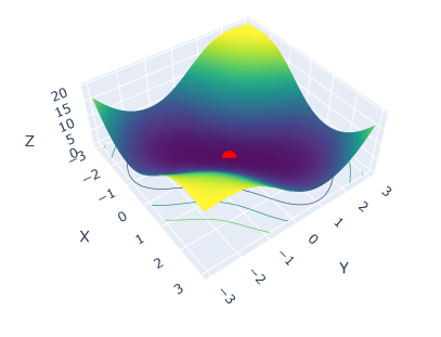
\includegraphics[width=\linewidth]{figures/2background/glob_min.png}
        \caption{A global minimum on \\
        $f(x,y) = (x-\sin(y))^2 + (y-\sin(x))^2$.}
        \label{fig:global_min}
    \end{subfigure}
    \hfill
    \begin{subfigure}[b]{0.48\linewidth}
        \centering
        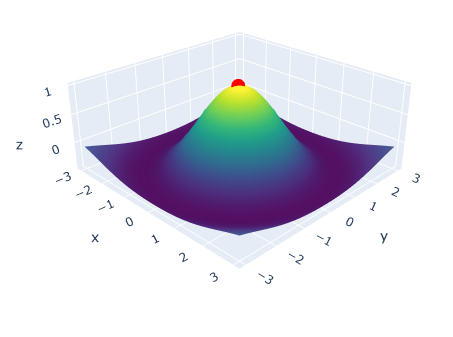
\includegraphics[width=\linewidth]{figures/2background/glob_max.png}
        \caption{A global maximum on \\
        $f(x,y) = \cos(x^2 + y^2) e^{-0.1 (x^2 + y^2)}$.}
        \label{fig:global_max}
    \end{subfigure}
    \caption{Examples of a global minimum and global maximum marked in red.}
    \label{fig:global_min_max}
\end{figure}

Finding such global optima is challenging, as we only have a limited set of information about $f$ and are resource constrained when evaluating it. Thus, many optimisation algorithms aim to find \textit{local optima}, which are points that are locally optimal. Similarly, there are \textit{local minimum} or \textit{local maximum} \citep{NoceWrig06, deep_learning_book}. We define these points with respect to a neighbourhood $\mathcal{N}$ of a point $x$. We provide examples in \cref{fig:local_min_max}.

\begin{definition}[Local Minimum]
    A point $x^*$ is a \textit{local minimum} if there exists a neighbourhood $\mathcal{N}$ around $x^*$ such that $f(x^*) \leq f(x)$ for all $x \in \mathcal{N}$. It is a \textit{strict local minimum} if instead $f(x^*) < f(x)$ for all $x \in \mathcal{N} \setminus \{x^*\}$.
\end{definition}

\begin{definition}[Local Maximum]
    A point $x^*$ is a \textit{local maximum} if there exists a neighbourhood $\mathcal{N}$ around $x^*$ such that $f(x^*) \geq f(x)$ for all $x \in \mathcal{N}$. It is a \textit{strict local maximum} if instead $f(x^*) > f(x)$ for all $x \in \mathcal{N} \setminus \{x^*\}$.
\end{definition}

\begin{figure}[h]
    \begin{subfigure}[b]{0.48\linewidth}
        \centering
        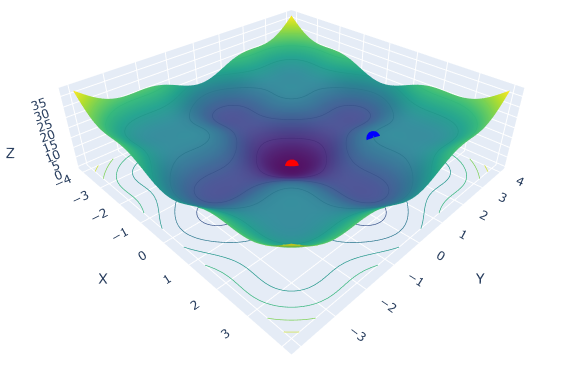
\includegraphics[width=\linewidth]{figures/2background/local_min.png}
        \caption{A local minimum on the egg crate function. \\
        $f(x,y) = (x^2 + y^2) + 5 (\sin(x)^2 + \sin(y)^2)$.
        }
        \label{fig:local_min}
    \end{subfigure}
    \hfill
    \begin{subfigure}[b]{0.48\linewidth}
        \centering
        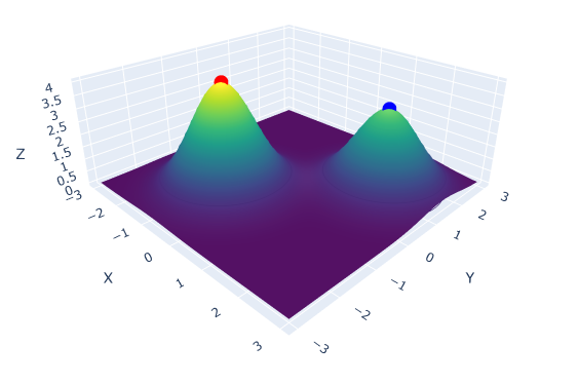
\includegraphics[width=\linewidth]{figures/2background/local_max.png}
        \caption{A local maximum on a multi-bump function. \\
        $f(x,y) = 3 e^{-(x-1.5)^2 - (y-1.5)^2} + \\
         4 e^{-(x+1)^2 - (y+1)^2} $.}
        \label{fig:local_max}
    \end{subfigure}
    \caption{Examples of a local minimum and local maximum marked in blue. The global minimum and global maximum are marked in red for comparison.}
    \label{fig:local_min_max}
\end{figure}

Beyond these, we have \textit{saddle points}. These are points that are locally flat but are neither a local minimum nor a local maximum, as seen in \cref{fig:saddle_point}. In any neighbourhood $\mathcal{N}$ around a saddle point, the function's value increases along some directions emanating from $x^*$ and decreases along others. We formally define saddle points in \cref{ssec:recognising_critical_points}.

\begin{figure}[h]
    \begin{subfigure}[b]{0.48\linewidth}
        \centering
        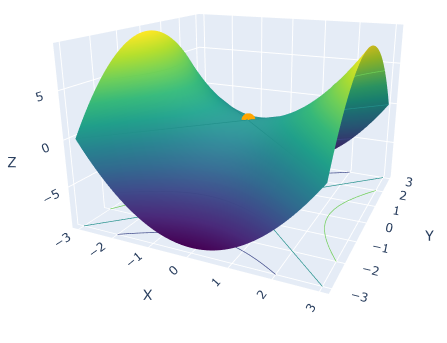
\includegraphics[width=0.8\linewidth]{figures/2background/horse_saddle.png}
        \caption{A saddle point on the horse saddle function. \\
        $f(x,y) = x^2 - y^2$.}
        \label{fig:horse_saddle}
    \end{subfigure}
    \hfill
    \begin{subfigure}[b]{0.48\linewidth}
        \centering
        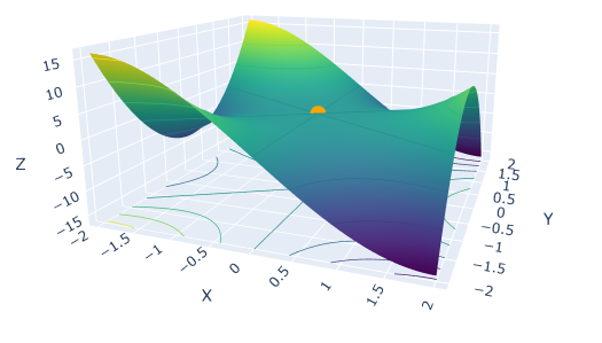
\includegraphics[width=\linewidth]{figures/2background/monkey_saddle.png}
        \caption{A saddle point on the monkey saddle function. \\
        $f(x,y) = x^3 - 3xy^2$.}
        \label{fig:monkey_saddle}
    \end{subfigure}
    \caption{Examples of two functions containing saddle points marked in orange.}
    \label{fig:saddle_point}
\end{figure}

\subsection{Recognising Critical Points}
\label{ssec:recognising_critical_points}

For smooth and differentiable functions, we can recognise critical points using the first and second order information about $f$. Here, we introduce the necessary and sufficient conditions that we use to do this. We restrict our attention to the class of functions that are twice continuously differentiable, where $f \in C^2$ \citep{NoceWrig06}.

% Nit: Jacobian or gradient here? [FIXED - gradient is good]
We start with a specific type of critical point, a \textit{stationary point}. A key property of any stationary point $x^*$ is that $f$ is locally flat at $x^*$. This implies that its gradient---the vector of \textit{first-order} partial derivatives, $\nabla f(x^*)$---must be zero \citep{deep_learning_book, mml_book}.
\begin{definition}[Stationary Point]
    A point $x^*$ is a \textit{stationary point} if $f$ is continuously differentiable at $x^*$ and its gradient is zero:
    \begin{align}
        \nabla f(x^*) = 0.
    \end{align}
\end{definition}

Given we are optimising $f$, we want to find a stationary point that is a local minimum. The following definition formalises the \textit{necessary first-order conditions} for a local minimum \citep{NoceWrig06}.
\begin{definition}[Necessary First-Order Conditions]
    If a point $x^*$ is a local minimum, and $f$ is continuously differentiable at $x^*$, then $\nabla f(x^*) = 0$ and $x^*$ is a stationary point.
\end{definition}

We note that all stationary points are critical points, but not all critical points are stationary points. For example, a function may have a critical point at a point where the gradient is undefined. A simple case is when $f(x) = \abs({x})$. This has a critical point at $x = 0$ where the gradient is undefined. However, given we restrict our attention to twice continuously differentiable functions, we do not need to consider these cases. 

% Nit: "Any nxn symmetric matrix A" and also specify that i < n etc. [FIXED]
All global optima, local optima, and saddle points are stationary points, but not all stationary points are optima. To distinguish between them, we examine the function's local curvature at $x^*$, which is captured by the \textit{Hessian matrix}---an $n \times n$ symmetric matrix of \textit{second-order} partial derivatives of $f$, denoted $\nabla^2 f(x)$ for a point $x$ \citep{deep_learning_book, mml_book, NoceWrig06}. We abbreviate the Hessian matrix for a function $f$ at a point $x$ as $H$ for convenience. The curvature information captured by $H$ can be summarised by its \textit{eigenvalues}. We denote the $i$-th eigenvalue of $H$, and more generally any $n \times n$ symmetric matrix $A$, as $\lambda_i$, where $i \in [1, n]$. We use these eigenvalues to characterise two important properties, \textit{positive semidefiniteness} and \textit{negative semidefiniteness}.

\begin{definition}[Positive Semidefinite Matrix]
    An $n \times n$ symmetric matrix $A$ is \textit{positive semidefinite} if all its eigenvalues are non-negative, where $\lambda_i \geq 0$ for all $i \in [1, n]$.
\end{definition}
\begin{definition}[Negative Semidefinite Matrix]
    An $n \times n$ symmetric matrix $A$ is \textit{negative semidefinite} if all its eigenvalues are non-positive, where $\lambda_i \leq 0$ for all $i \in [1, n]$.
\end{definition}

These properties can now be used to formalise the \textit{necessary second-order conditions} to classify stationary points \citep{NoceWrig06}. We write these for a local minimum as follows.
\begin{definition}[Necessary Second-Order Conditions]
    If a point $x^*$ is a local minimum, and $f$ is twice continuously differentiable, then:
    \begin{itemize}
        \item $\nabla f(x^*) = 0$
        \item $H$ is positive semi-definite at $x^*$.
    \end{itemize}
    \label{definition:second_order_necessary}
\end{definition}
Similarly, the above definition can be extended to a local maximum when $H$ is negative semi-definite.

% Nit: Indefinite matrix definition can have +,- or 0 eigenvalues. [FIXED]
A special case is when $H$ is \textit{indefinite}.
\begin{definition}[Indefinite Matrix]
    An $n \times n$ symmetric matrix $A$ is \textit{indefinite} if it is not positive semidefinite and not negative semidefinite. That is, there exists $\lambda_i > 0$ and $\lambda_j < 0$ for some $i, j \in [1, n]$.
\end{definition}
Here, the function curves upwards in some directions and downwards in others. This is a saddle point.

\begin{definition}[Saddle Point]
    A stationary point $x^*$ is a \textit{saddle point} if $H$ is indefinite at $x^*$.
\end{definition}

% Nit: Give example of strict local maximum that's guaranteed to decrease versus a flat region that's a local maximum.
Now, we can classify between local minima, local maxima, and saddle points based on whether $H$ is positive/negative semi-definite or indefinite. However, we can still fall short of distinguishing between local minima/maxima and strict local minima/maxima. For example, if $H$ is positive semidefinite at $x^*$, $x^*$ could be a local minimum or a flat region that is not a strict minimum \citep{NoceWrig06}. Similarly, if $H$ is negative semidefinite at $x^*$, we could be in a local maximum or a flat region. To distinguish between this, we consider two further properties---\textit{positive definiteness} and \textit{negative definiteness}, which are stronger conditions than positive and negative semi-definiteness.

\begin{definition}[Positive Definite Matrix]
    An $n \times n$ symmetric matrix $A$ is \textit{positive definite} if all its eigenvalues are positive, where $\lambda_i > 0$ for all $i \in [1, n]$.
\end{definition}
\begin{definition}[Negative Definite Matrix]
    An $n \times n$ symmetric matrix $A$ is \textit{negative definite} if all its eigenvalues are negative, where $\lambda_i < 0$ for all $i \in [1, n]$.
\end{definition}

We can now guarantee something stricter about the nature of $x^*$, that it is a strict local minimum/maximum. This guarantees that we will optimise our objective without being trapped in a flat region. We write these as the \textit{sufficient second-order conditions} for optimisation \citep{NoceWrig06}. We formalise this for a strict local minimum as follows.
\begin{definition}[Sufficient Second-Order Conditions]
    If $f$ is twice continuously differentiable, and $\nabla f(x^*) = 0$, and $H$ is positive definite at $x^*$, then $x^*$ is a strict local minimum.
    \label{definition:second_order_sufficient}
\end{definition}
Similarly, we can write the sufficient second-order conditions for a strict local maximum when $H$ is negative definite at $x^*$.

We note that the sufficient second-order conditions are not necessary. A point $x^*$ may satisfy the necessary second-order conditions but fail to satisfy the sufficient second-order conditions \citep{NoceWrig06}. For example, the function $f(x) = x^4$ has a strict local minimum at $x^* = 0$, but $H$ vanishes here and is thus not positive definite at $x^*$. 

\subsection{Convexity}
\label{ssec:convexity}

The property of convexity simplifies the task of finding optima. A function $f$ is \textit{convex} if geometrically, the line segment connecting any two points on the function's graph lies on or above the graph itself \citep{cvbook, NoceWrig06, mml_book}. We provide an illustration in \cref{fig:convex_function}, and formally define this as follows.

% Nit: Define convex set here? [FIXED - just mention it with a domain D]
% [REVISE]
\begin{definition}[Convex Function]
    A function $f: D \to \mathbb{R}$, where $D \subseteq \mathbb{R}^n$ is a convex set, is \textit{convex} if for any two points $x_1, x_2$ in its domain, and any scalar $t \in [0, 1]$:
    \begin{align}
        f(t x_1 + (1-t)x_2) \leq t f(x_1) + (1-t)f(x_2).
    \end{align}
    This is a special case of \textit{Jensen's inequality}. Equivalently, a function is convex if $H$ is positive semidefinite for all $x$ in the domain of $f$ given $f$ is twice continuously differentiable.
\end{definition}

% Nit: Image resizing [FIXED]
\begin{figure}[h]
    \centering
    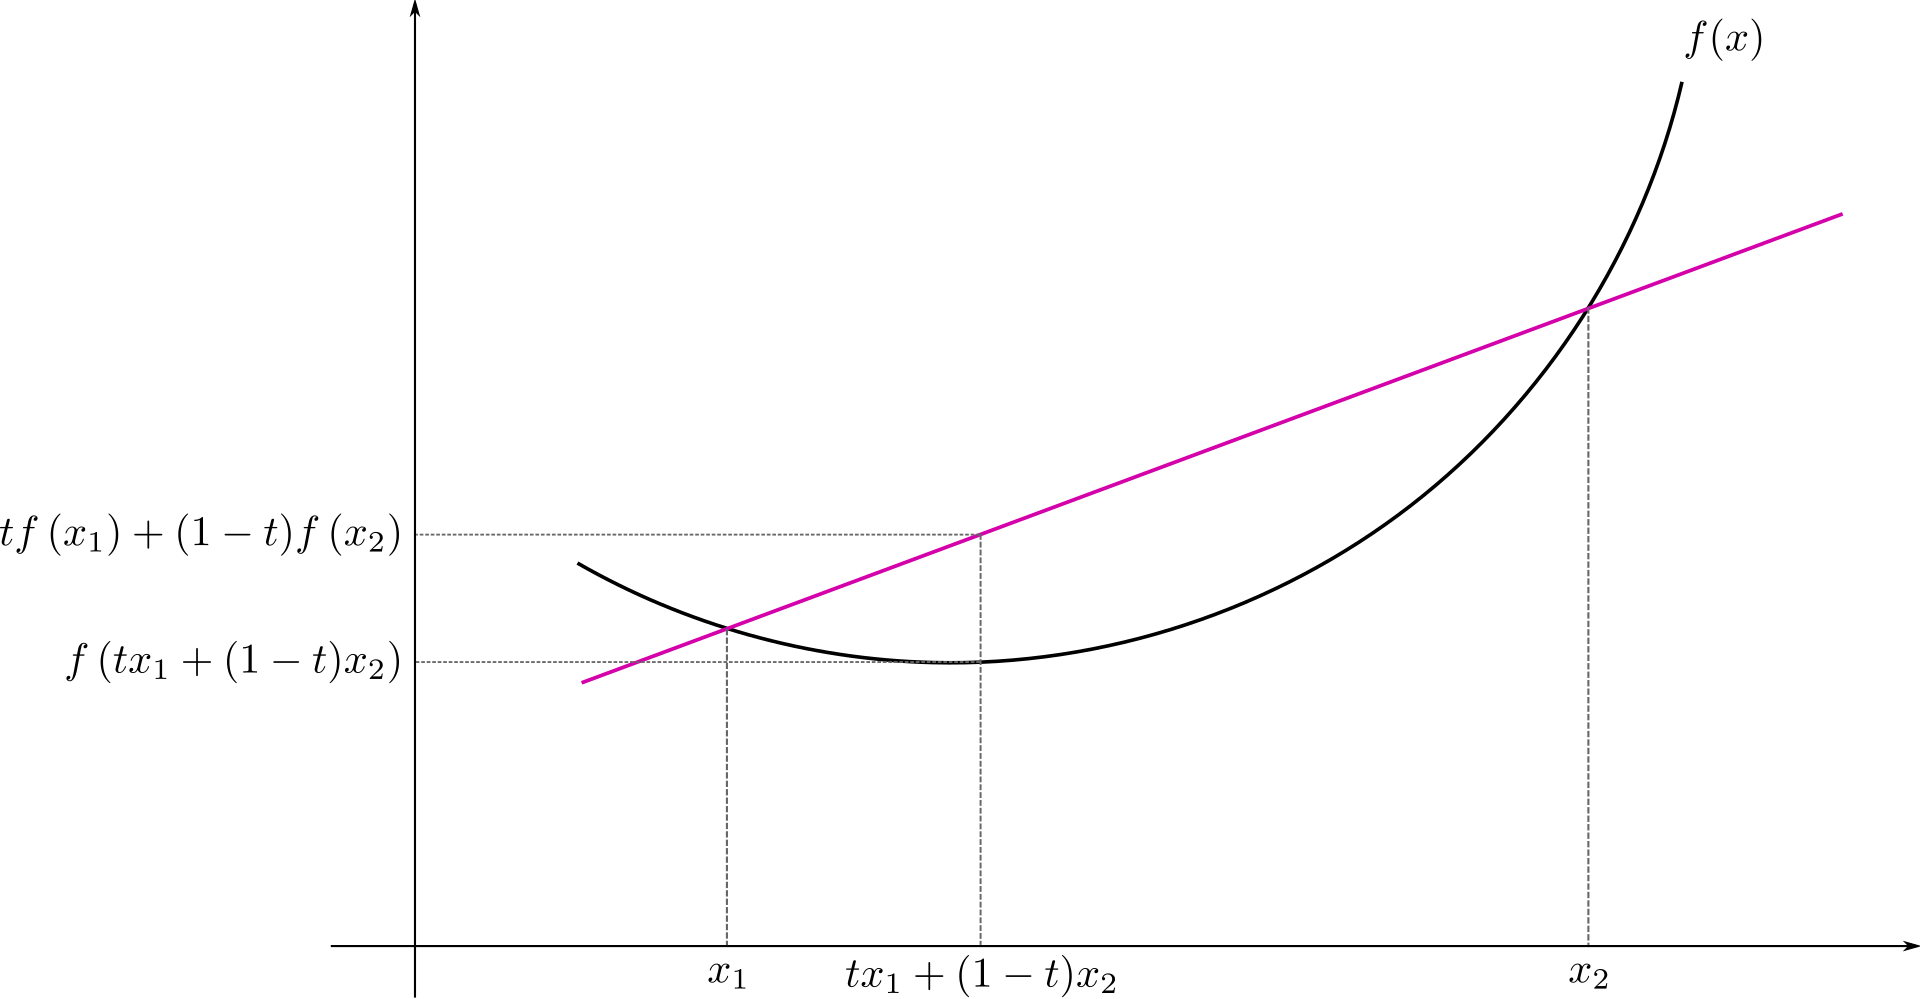
\includegraphics[width=0.9\linewidth]{figures/2background/ConvexFunction.svg.png}
    \caption{An illustration of a convex function. The line segment created by $x_1$ and $x_2$ clearly lies above the function.}
    \label{fig:convex_function}
\end{figure}

Convex functions are particularly appealing because they possess global properties that simplify the optimisation process. We call these properties the \textit{global optimality conditions} for convex functions \citep{cvbook, NoceWrig06}.

\begin{definition}[Global Optimality Conditions for Convex Functions]
    If $f$ is convex, then: 
    \begin{itemize}
        \item Any local minimum $x^*$ is a global minimum of $f$.
        \item Any stationary point $x^*$ is a global minimum of $f$ given $f$ is continuously differentiable.
    \end{itemize}
\end{definition}

This means that if we find a stationary point of a convex function, we have found the overall best possible solution. Additionally, given that $H$ is guaranteed to be positive semidefinite for twice continuously differentiable convex functions, certain optimisation algorithms can guarantee convergence to a global minimum regardless of the initialisation point. 

We can further strengthen this by considering the property of \textit{strict convexity}. A strictly convex function is one where the line segment connecting any two points on the function's graph lies strictly above the graph between those points \citep{cvbook, NoceWrig06}. We illustrate the difference between convex and strictly convex functions in \cref{fig:diff_geometric_convexity}. Formally, we define strictly convex functions as follows.
\begin{definition}[Strictly Convex Function]
    A function $f: \mathbb{R}^n \to \mathbb{R}$ is \textit{strictly convex} if its domain is a convex set, and for any two distinct points $x_1, x_2$ such that $x_1 \neq x_2$ in its domain, and any scalar $t \in (0, 1)$:
    \begin{align}
        f(t x_1 + (1-t)x_2) < t f(x_1) + (1-t)f(x_2).
    \end{align}
    Equivalently, a function is strictly convex if $H$ is positive definite for all $x$ in the domain of $f$ given $f$ is twice continuously differentiable.
\end{definition}

% Nit: Make the ReLU one a bit more dark - it's hard to see the line. [FIXED]
\begin{figure}[h]
    \begin{subfigure}[b]{0.48\linewidth}
        \centering
        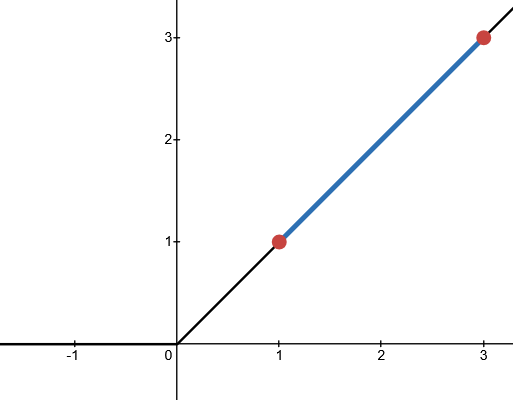
\includegraphics[width=0.8\linewidth]{figures/2background/relu.png}
        \caption{The Rectified Linear Unit (ReLU) function, $f(x) = \max(0, x)$, is convex, but not strictly convex since we can pick two points where the line segment is not strictly above the function.}
        \label{fig:convex_relu}
    \end{subfigure}
    \hfill
    \begin{subfigure}[b]{0.48\linewidth}
        \centering
        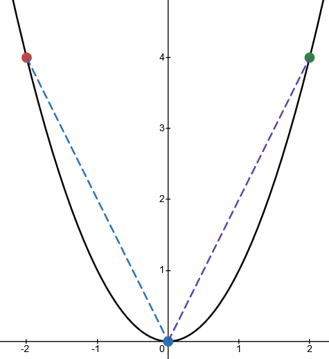
\includegraphics[width=0.6\linewidth]{figures/2background/parabola.png}
        \caption{The parabola function, $f(x) = x^2$, is strictly convex since for any two points, the line segment will always lie above the function.}
        \label{fig:strict_convex_parabola}
    \end{subfigure}
    \caption{The geometrical difference between a convex function and a strictly convex function.}
    \label{fig:diff_geometric_convexity}
\end{figure}

Strictly convex functions are a subset of convex functions. They inherit the same global optimality conditions, but with an additional \textit{uniqueness} property that makes them incredibly easy to optimise \citep{NoceWrig06}.
\begin{definition}[Uniqueness of Global Minimum]
    If $f$ is strictly convex, then there exists \textit{at most one} local minimum of $f$. Consequently, if it exists, then it is the global minimum of $f$.
\end{definition}
Thus, if we find any stationary point of a strictly convex function, we have found the global minimum \citep{NoceWrig06}. This is different from convex functions, where there could be multiple global minima. We provide an illustration of this in \cref{fig:diff_convex_functions}. This makes strictly convex functions extremely desirable for optimisation, since we have a guaranteed unique solution.

\begin{figure}[h]
    \begin{subfigure}[b]{0.48\linewidth}
        \centering
        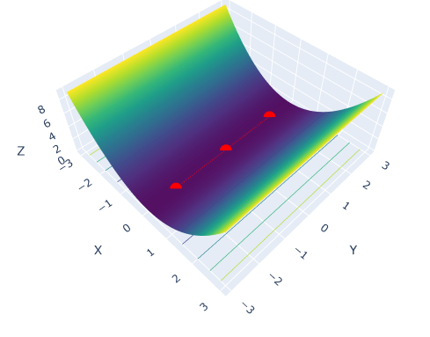
\includegraphics[width=0.8\linewidth]{figures/2background/convex_func.png}
        \caption{Multiple global minima on the convex function
        $f(x,y) = x^2$.}
        \label{fig:convex_func}
    \end{subfigure}
    \hfill
    \begin{subfigure}[b]{0.48\linewidth}
        \centering
        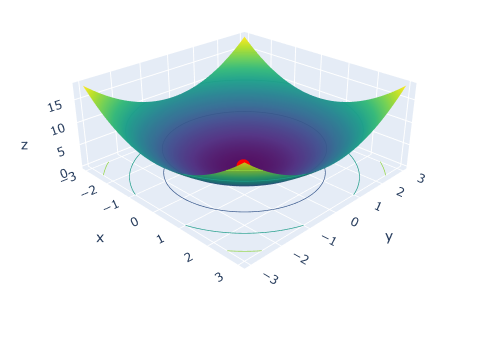
\includegraphics[width=\linewidth]{figures/2background/strict_convex.png}
        \caption{A unique global minimum on the strictly convex function
        $f(x,y) = x^2 + y^2$.}
        \label{fig:strict_convex_func}
    \end{subfigure}
    \caption{The difference between a convex function with multiple global minima and a strictly convex function with a unique global minimum.}
    \label{fig:diff_convex_functions}
\end{figure}


\subsection{Ill-Conditioning and Non-Smoothness}
\label{ssec:ill_conditioning_nonsmooth}

While convexity simplifies the optimisation process, two other characteristics, \textit{ill-conditioning} and \textit{non-smoothness}, significantly increase the difficulty instead. We now discuss these two characteristics and their influence the optimisation landscape.


% Nit:
% - We introduce condition number based on H that is strictly convex for f, but then go on to use the Rosenbrock to demonstrate ill-conditioning with the perturbations. [FIXED]
% - We also don't show how H influences the perturbations for this, but just show an example. [FIXED - Don't think this matters and is unnecessary. It is good how it is.]
% TODO - Reference the second-order methods which tackle this.
\subsubsection{Ill-Conditioning}
\label{sssec:ill_conditioning}

An optimisation problem is \textit{ill-conditioned} if the objective function $f$ is highly sensitive to small changes to its parameters in the vicinity of a solution $x^*$. Geometrically, this corresponds to a landscape that is either elongated with narrow valleys, or steep ridges with large dropoffs, as illustrated in \cref{fig:ill_conditioned_functions}. To motivate the problem of ill-conditioning, we consider the deterministic Rosenbrock function
\begin{align}
    f(x,y) = (1 - x)^2 + 100(y - x^2)^2.
    \label{eq:rosenbrock_function}
\end{align}
The global minimum for this function is at $(x,y) = (1,1)$. Suppose we introduce a small perturbation $\epsilon_1 = 0.01$ to $x$ and $\epsilon_2 = 0.02$ to $y$ around the minimum. Our function evaluates to
\begin{align}
    f(x + \epsilon_1, y + \epsilon_2) = f(1 + 0.01, 1 + 0.02)
    \approx 1e-4.
\end{align}
If we modify the perturbations to $\epsilon_1 = 0.02$ and $\epsilon_2 = -0.01$ instead, our function value now becomes
\begin{align}
    f(x + \epsilon_1, y + \epsilon_2) = f(1 + 0.02, 1 - 0.01)
    \approx 0.25.
\end{align}

\begin{figure}[h]
    \begin{subfigure}[b]{0.48\linewidth}
        \centering
        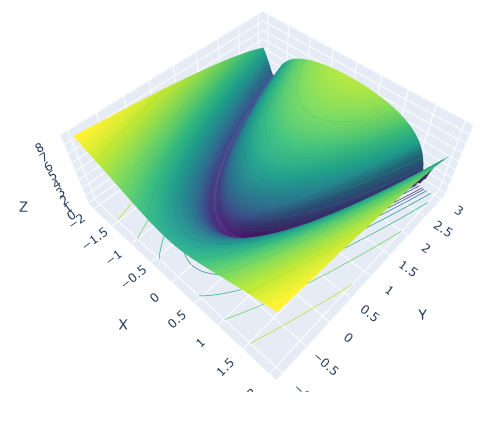
\includegraphics[width=\linewidth]{figures/2background/rosenbrock.png}
        \caption{The deterministic Rosenbrock function \\ 
        $f(x,y) = (1-x)^2 + 100(y-x^2)^2$}
        \label{fig:rosenbrock}
    \end{subfigure}
    \hfill
    \begin{subfigure}[b]{0.48\linewidth}
        \centering
        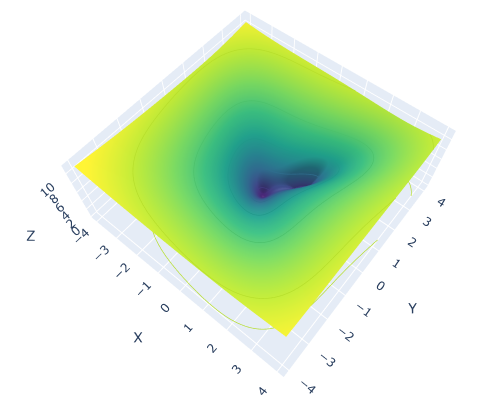
\includegraphics[width=\linewidth]{figures/2background/wood_func.png}
        \caption{A simplified 2D analogue of the wood function \\
        $f(x,y) = 100*(y - x^2)^2 + (1 - x)^2 + 90*(y^2 - x)^2 + (1 - y)^2$}
        \label{fig:wood_function}
    \end{subfigure}
    \caption{The optimisation landscape of two ill-conditioned functions. The Rosenbrock function (left) shows the narrow valley towards the minimum, whereas the 2D wood function (right) shows a steep dropoff as we approach the minimum.}
    \label{fig:ill_conditioned_functions}
\end{figure}

We see a significant change in how our function behaves, where it is now $2500$ times larger than before with only small changes applied to its input. This illustrates the problem of ill-conditioning, which makes it difficult for optimisation algorithms to converge to a solution. We describe the ill-conditioning of a problem in terms of the \textit{condition number} \citep{regression_book, cvbook}.

% Nit: Be consistent with the notation when you previously defined the eigenvalues before. [FIXED]
\begin{definition}[Condition Number]
    For any non-singular square matrix $A \in \mathbb{R}^{n \times n}$, its \textit{condition number} with respect to a given matrix norm $||\cdot||$ is defined as:
    \begin{align}
        \kappa(A) = ||A||\cdot||A^{-1}||,
    \end{align}
    In the context of optimisation, if $f$ is twice continuously differentiable at $x$ and $H$ is positive definite at $x$, then the condition number is the ratio of the largest eigenvalue $\lambda_{\max}$ to the smallest eigenvalue $\lambda_{\min}$ of $H$ under the spectral norm $|| \cdot ||_2$. 
    \begin{align}
        \kappa(H) = ||H||_2||H^{-1}||_2 = \lambda_{\max}(H)\lambda_{\max}(H^{-1}) = \lambda_{\max}(H) \cdot \frac{1}{\lambda_{\min}(H)} = \frac{\lambda_{\max}(H)}{\lambda_{\min}(H)}.
    \end{align}
\end{definition}

In the Rosenbrock example, the condition number is $2508$ at the minimum, which explains the behaviour we observed. Ill-conditioning poses significant challenges for many optimisation algorithms, especially those relying on gradient information. In these landscapes, finding solutions that are robust to perturbations is difficult. Algorithms may get stuck and make excessively small steps to counteract the ill-conditioning, which slows convergence, or they become unstable due to taking overly aggressive steps. Efficient navigation of these landscapes require algorithms to be \textit{scale invariant} \citep{NoceWrig06}. We discuss these algorithms in more detail in \cref{sec:optimisation_in_deep_learning}.

\subsubsection{Non-Smooth Problems}
\label{sssec:non_smooth_problems}

So far, we have talked about optimisation problems where the objective function $f$ is smooth and usually twice continuously differentiable. However, many optimisation problems that we encounter, particularly in machine learning, involve \textit{non-smooth functions}. These are functions that possess points at which the function or its derivatives are not well-defined. We provide an example of such functions which have points of non-differentiability in \cref{fig:non_smooth_functions}. 

\begin{figure}[h]
    \begin{subfigure}[b]{0.48\linewidth}
        \centering
        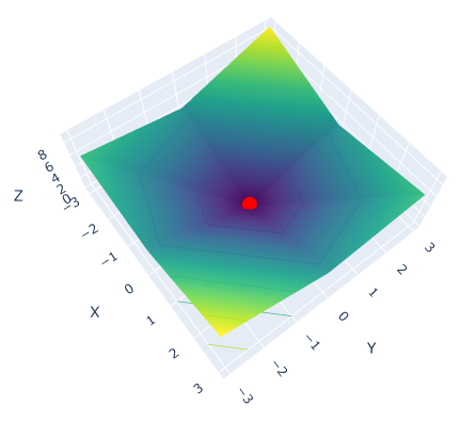
\includegraphics[width=\linewidth]{figures/2background/abs_func.png}
        \caption{The function
        $f(x, y) =\abs(x) + \abs(y)$ has an undefined gradient at (0,0).}
        \label{fig:abs_function}
    \end{subfigure}
    \hfill
    \begin{subfigure}[b]{0.48\linewidth}
        \centering
        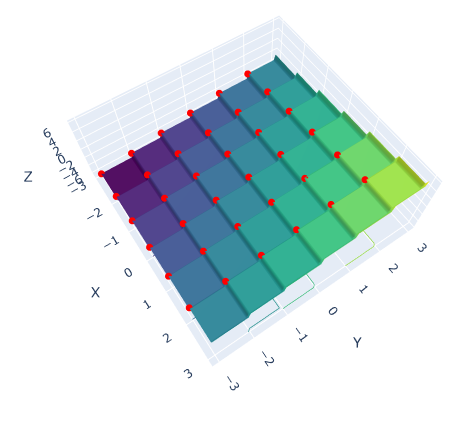
\includegraphics[width=\linewidth]{figures/2background/floor_func.png}
        \caption{The step function
        $f(x,y) = \lfloor x \rfloor + \lfloor y \rfloor$ has undefined gradients at all integer points.}
        \label{fig:step_function}
    \end{subfigure}
    \caption{The optimisation landscape of two non-smooth functions, with points of non-differentiability highlighted in red.}
    \label{fig:non_smooth_functions}
\end{figure}

Non-smoothness is common in machine learning, with terms such as ReLU and L1 regularisation being used in many problem settings \citep{deep_learning_book, mml_book}. At points of non-differentiability, classical optimisation concepts that we have been discussing break down. The optimisation of non-smooth functions requires alternative theoretical frameworks and algorithms. While this is out of scope for this thesis, we briefly provide an overview of such methods in 
\cref{chap:lit_review}. In specific instances, we can reformulate the non-smooth problem into a smooth approximation. For example, the ReLU function has an equivalent smooth approximation given by the Softplus function, $f(x) = \log(1 + e^x)$ \citep{deep_learning_book} \citep{pytorch}. While non-smooth optimisation is out of scope for this thesis, we provide an overview of such methods in \cref{chap:lit_review}.

% Nit: I don't think this is relevant it's just showing both activation functions. [FIXED]
% \begin{figure}[h]
%     \centering
%     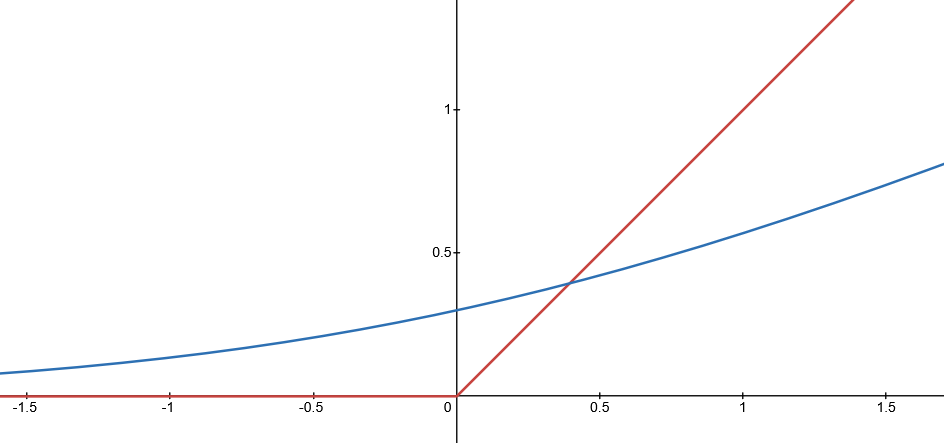
\includegraphics[width=0.8\linewidth]{figures/2background/relu_softplus.png}
%     \caption{The ReLU function (red) and its smooth approximation, the Softplus function (blue), given by $f(x) = \log(1 + e^x)$. The ReLU function is non-differentiable at $x = 0$, but the Softplus function is differentiable everywhere.}
%     \label{fig:relu_softplus}
% \end{figure} 

\section{Optimisation in Deep Learning}
\label{sec:optimisation_in_deep_learning}

% Nit: Is this actually necessary to include? I'm not sure if we'll use this notation in the thesis? [FIXED]
% Nit: Input data is R^n, and model parameters are R^n - clash? [FIXED]
% Nit: Include minibatches or batches? [FIXED - Don't need, just sample]
Deep learning introduces a new set of challenges to the optimisation landscape. In deep learning, we usually have a set of \textit{input data} $x \in \mathbb{R}^n$ and a \textit{target output} $y \in \mathbb{R}^m$. Our goal is to learn a mapping from $x$ to $y$. This is represented by a \textit{model}, which is a complex, highly parameterised function that is usually non-convex and can be thought of as a \textit{universal function approximator} \citep{universal_func_approx}. Through exposure to many examples in a \textit{training set}, the model makes \textit{predictions} $\hat{y}$ for inputs $x$, and is then evaluated on a \textit{test set} with new, unseen inputs. Ideally, we would like our model to make accurate predictions on the test set, as this is a good indicator of generalisation performance. We optimise the model's \textit{parameters}, $\theta \in \mathbb{R}^N$, by minimising a real-valued \textit{loss function} $L: \mathbb{R}^N \to \mathbb{R}$ that measures model's performance. Typically, this is written as an average over the training set, such as
\begin{align}
    L(\theta) = \mathbb{E}_{(x, y) \sim \hat{p}_{data}} \mathcal{L}(f(x; \theta), y) = \mathbb{E}_{(x, y) \sim \hat{p}_{data}} \ell(\hat{y}, y),
    \label{eq:loss_function}
\end{align}
where $\hat{y} = f(x; \theta)$, $\mathcal{L}$ is the per-example loss (such as mean-squared error or cross-entropy), and $\hat{p}_{data}$ is the empirical distribution of our training set. In practice, we usually sample a set of examples $X_i, Y_i$ from the training set to compute $\hat{y_i}$ and $L$ \citep{deep_learning_book, pytorch}. We provide a general algorithm for deep learning optimisation in \cref{alg:general_deep_learning_algo}.

\begin{algorithm}[H]
    \DontPrintSemicolon
    \KwIn{Training data $\{(x_i, y_i)\}_{i=1}^{n}$, model $f(x; \theta)$ with initial parameters $\theta_0$, loss function $\mathcal{L}$, number of iterations $T$}
    \KwOut{Optimised parameters $\theta$}
    $\theta \leftarrow \theta_0$\;
    \For{$t = 1, 2, \ldots, T$}{
        Sample a set of examples $(X_t, Y_t)$ from training data\;
        Compute loss $L_t(\theta) = \mathcal{L}(f(X_t; \theta), Y_t)$\;
        Find an update direction $\Delta\theta$\;
        $\theta \leftarrow \theta + \Delta\theta$\;
    }
    \Return{$\theta$}
    \caption{General Model Optimisation}
    \label{alg:general_deep_learning_algo}
\end{algorithm}


We limit our discussion of $\mathcal{L}$ to the \textit{supervised} learning case, where we have a fixed input $x$ and a corresponding target output $y$ and the inputs to $\mathcal{L}$ are $\hat{y}$ and $y$. It is easy to extend this development to the \textit{regularised} case, for example by including $\theta$ as an argument, or the \textit{unsupervised} case by removing $y$. 

In this section, we discuss the challenges of optimisation in deep learning. We start by discussing the behaviour of high-dimensional landscapes in \cref{ssec:dl_challenges}. This is followed by a discussion of first-order methods in \cref{ssec:first_order_methods} and second-order methods in \cref{ssec:second_order_methods}.

\subsection{Challenges in High-Dimensional Landscapes}
\label{ssec:dl_challenges}

% TODO: Needs more rigorous citing - see 8.2 of the deep learning book and copy those references.
High-dimensional landscapes are complex and difficult to navigate. Recall that we saw an example of this with a highly parameterised high-dimensional ResNet model in \cref{chap:introduction}. The geometric intuition derived from low-dimensional spaces is usually not applicable. We observe two key properties in high-dimensions.
\begin{itemize}
    \item \textit{Proliferation of saddle points}: Saddle points are \textit{exponentially} more likely than local minima as dimensionality $N$ increases \citep{dauphin2014sfn}.
    \item \textit{Local minima are close to global minimum}: Local minima in high dimensions are likely to have values very close to the global minimum \citep{dauphin2014sfn,choromanska2015loss}.
\end{itemize}

% TODO: Needs ref here for the Wigner bit. [FIXED]
We can understand the first property by analysing $H$ in the context of our loss function, where we now have that $H = \nabla^2 L(\theta)$. As established in \cref{ssec:recognising_critical_points}, a local minimum requires all $H$ to be positive semidefinite, in which all eigenvalues are greater than or equal to zero. A saddle point however possesses both positive and negative eigenvalues. We note that for large random Gaussian matrices, the eigenvalue distribution follows \textit{Wigner's semicircle law}, which states that as $N$ increases, we observe the following \citep{wigner1958distribution, dauphin2014sfn}.
\begin{itemize}
    \item An eigenvalue $\lambda_i$ has an equal probability of $\frac{1}{2}$ to be positive or negative. 
    \item Each eigenvalue's probability is approximately independent of others.
\end{itemize}

\begin{figure}[h]
    \begin{subfigure}[b]{0.48\linewidth}
        \centering
        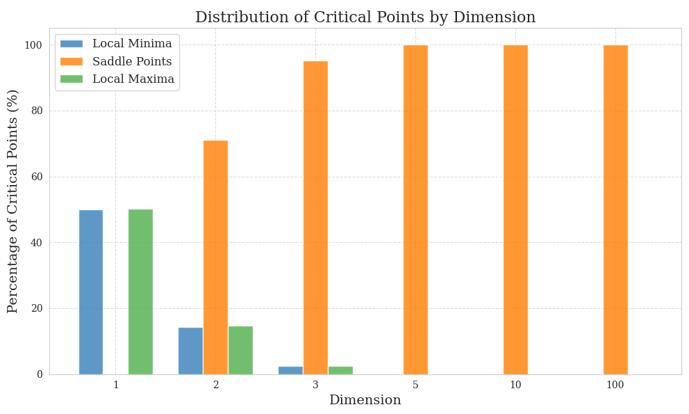
\includegraphics[width=\linewidth]{figures/2background/critical_dist.png}
        \caption{The distribution of local minima, local maxima, and critical points of random Gaussian matrices of dimensions $N$.}
        \label{fig:critical_dist}
    \end{subfigure}
    \hfill
    \begin{subfigure}[b]{0.48\linewidth}
        \centering
        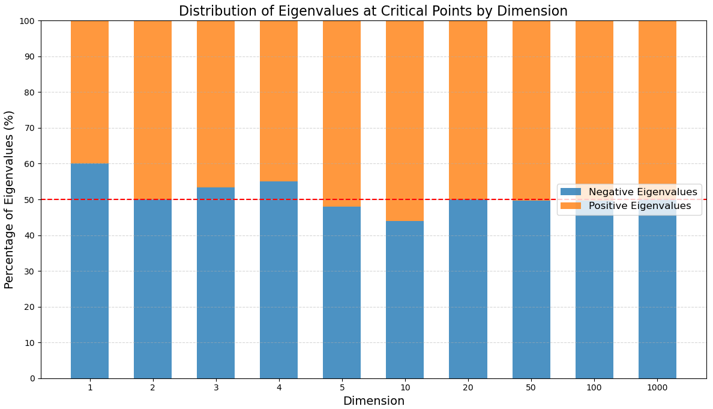
\includegraphics[width=\linewidth]{figures/2background/eigen_dist.png}
        \caption{The distribution of the eigenvalues at critical points for various random Gaussian matrices of dimensions $N$.}
        \label{fig:eigen_dist}
    \end{subfigure}
    \caption{The distribution of critical points and their eigenvalues for random Gaussian matrices of dimensions $N$.}
    \label{fig:high_dim_experiment}
\end{figure}

% TODO: Citations for the experiments part. [FIXED]
Intuitively, we can consider the probability of each eigenvalue as akin to an independent fair coin toss. The probability of obtaining $N$ non-negative eigenvalues diminishes exponentially with increasing $N$. The same goes for obtaining $N$ non-positive eigenvalues. Consequently, obtaining $N$ eigenvalues with mixed signs are far more probable, which explains the proliferation of saddle points, as seen in \cref{fig:critical_dist}. As $N$ increases, the eigenvalues follow the distribution of the semicircle law more, and we get approximately equal numbers of positive and negative eigenvalues. We see this in \cref{fig:eigen_dist}. While we have this case for large random Gaussian matrices, we note that this applies to the deep learning setting as well. Experimental evidence shows that the landscapes of deep learning models display many more saddle points than local minima \citep{dauphin2014sfn}. We provide a more detailed analysis of the deep learning optimisation landscape in \cref{chap:evaluation}.

% TODO: Citations and Deep Learning Book chapter 8 ref here.
The second property follows as a direct consequence of the first. Suppose we consider a local minima with a function value that is substantially higher than the global minimum. Given high dimensionality, it is very probable that there exists at least one eigenvalue that is negative which we can take to minimise the objective in some immediate neighbourhood. Such a point would then be a saddle point, offering a local escape direction. Given that local minima are so rare, we observe that they can only take a range of loss values, in which these are close to the global minimum \citep{choromanska2015loss, dauphin2014sfn, deep_learning_book}. This suggests that the challenge in deep learning optimisation is less about getting trapped in poor local minima and more about efficiently navigating the numerous saddle points that dominate the landscape \citep{deep_learning_book}. 

The dominance of saddle points changes the optimisation landscape and impedes the progress of optimisation algorithms. First-order methods that rely on gradient information, such as \textit{gradient descent}, experience slowed convergence in these regions. Second-order methods such as \textit{Newton's method} also face problems, as in some cases they are actually attracted to saddle points, even though they have the benefit of having local curvature information and are scale invariant. We cover these in the next two sections \cref{ssec:first_order_methods} and \cref{ssec:second_order_methods}.

% Nit: Both these sections need a generic algorithm showing the update rules being applied. [FIXED - has a general update before]
\subsection{First-Order Methods}
\label{ssec:first_order_methods}

Most optimisation algorithms in deep learning are \textit{first-order methods}. First-order optimisation involves using the \textit{gradient of the loss function} to iteratively update the model parameters $\theta$ \citep{deep_learning_book, mml_book}. In the deep learning setting, this is defined as the vector of partial derivatives of $L$ with respect to $\theta$ \citep{deep_learning_book}.
\begin{definition}[Gradient of the Loss Function]
    The gradient of the loss function $L$ with respect to the parameters $\theta$ is defined as:
    \begin{align}
        \nabla L(\theta) = \left(\frac{\partial L}{\partial \theta_1}, \frac{\partial L}{\partial \theta_2}, \ldots, \frac{\partial L}{\partial \theta_N}\right).
    \end{align}
\end{definition}

We abbreviate this as $g$ for brevity. The gradient vector points in the direction of steepest ascent of the loss function, and is thus the direction of most rapid change. We perform an optimisation step by moving in the \textit{negative gradient} direction, which is the direction of \textit{steepest descent} \citep{deep_learning_book, mml_book, NoceWrig06}. The general update rule is given by:
\begin{align}
    \Delta \theta &= - \alpha_t g_t, \\
    \theta_{t+1} &= \theta_t + \Delta \theta,
    \label{equation:first_order_update}
\end{align}
where $\theta_t$ denotes the model parameters at iteration $t$, $g_t$ is the gradient evaluated at that point, and $\alpha_t > 0$ is the \textit{learning rate}. The learning rate controls the step size of the steepest descent step.

First-order methods are computationally efficient and scalable. This is because the update can be performed with $O(N)$ space for a model with $N$ parameters for a single sample of data \citep{deep_learning_book, mml_book}. This makes them extremely appealing for deep learning, where models have millions or even billions of parameters and we have constraints on computational resources \citep{deep_learning_book}. These methods are also highly parallelisable \citep{pytorch}. Modern GPU hardware and distributed computing with efficient low-level kernels enable gradient computations to be executed across multiple processing units, making them even more appealing \citep{pytorch}.

However, while simple and effective in many scenarios, the reliance of first-order methods on the gradient becomes problematic in high-dimensional landscapes that are characterised by a proliferation of saddle points, as briefly mentioned in \cref{ssec:dl_challenges}. In these regions of low curvature, the gradient magnitude is small. This leads to small, incremental updates to our parameters that result in slowed convergence. Conversely, in ill-conditioned landscapes as discussed in \cref{ssec:ill_conditioning_nonsmooth}, the gradient can be noisy and unstable. 
This is particularly the case for some ill-conditioned problems, such as the \textit{Rahimi-Recht function}, where the landscape becomes increasingly steep and majority of the eigenvalues tend towards infinity as we approach the minimum \citep{recht2017kitchen}. This results in slowed convergence and suboptimal solutions being found, and we see this in the next section in \cref{fig:scale_invariance}. In the worst case, the possibility of divergence is also present, which we will see later on in our evaluation in \cref{chap:evaluation}. 

Numerous variations of first-order methods, despite these challenges, have made them successful in deep learning and cemented them as the current state-of-the-art. These include the use of \textit{stochastic gradients}, \textit{momentum}, and \textit{adaptive} methods \citep{monro1990stochastic, kingma2014adam}. We provide a comprehensive overview of these optimisation algorithms in \Cref{chap:lit_review}.

\subsection{Second-Order Methods}
\label{ssec:second_order_methods}

% Nit: Re-define H as mathbb{H} instead
Second-order methods use local curvature information to traverse the optimisation landscape. This is captured by the \textit{Hessian of the loss function}, which is in contrast to first-order methods that solely rely on the gradient. We introduced the Hessian generally in \cref{ssec:recognising_critical_points}. Here, we define it in the context of deep learning, where it is the matrix of second-order partial derivatives of $L$ with respect to the parameters $\theta$ \citep{deep_learning_book}.
\begin{definition}[Hessian of the Loss Function]
    The Hessian of the loss function $L$ with respect to the parameters $\theta$ is the $N \times N$ matrix of second-order partial derivatives:
    \begin{align}
        \nabla^2 L(\theta) = \left(\frac{\partial^2 L}{\partial \theta_i \partial \theta_j}\right)_{i,j=1}^N = 
        \begin{pmatrix}
            \frac{\partial^2 L}{\partial \theta_1^2} & \frac{\partial^2 L}{\partial \theta_1 \partial \theta_2} & \cdots & \frac{\partial^2 L}{\partial \theta_1 \partial \theta_N} \\
            \frac{\partial^2 L}{\partial \theta_2 \partial \theta_1} & \frac{\partial^2 L}{\partial \theta_2^2} & \cdots & \frac{\partial^2 L}{\partial \theta_2 \partial \theta_N} \\
            \vdots & \vdots & \ddots & \vdots \\
            \frac{\partial^2 L}{\partial \theta_N \partial \theta_1} & \frac{\partial^2 L}{\partial \theta_N \partial \theta_2} & \cdots & \frac{\partial^2 L}{\partial \theta_N^2}
        \end{pmatrix}.
    \end{align}
\end{definition}
We denote this as $H$ for brevity. Note that from here onwards, $H$ specifically refers to $\nabla^2 L(\theta)$ rather than the general Hessian $\nabla^2 f(x)$ of an objective function previously defined in \cref{ssec:recognising_critical_points}.

The foundation of many second-order methods is the approximation of the loss function using a \textit{quadratic model} \citep{NoceWrig06}. This is derived by taking a second-order \textit{Taylor expansion} of the loss function \citep{NoceWrig06}. We define a Taylor expansion in the one dimensional case as follows.
\begin{definition}[Taylor Expansion]
    Given a function $f: \mathbb{R} \to \mathbb{R}$ where $f \in C^p$, that is $f$ is $p$ times continuously differentiable, the Taylor expansion of $f$ about $x = a$ is given by:
    \begin{align}
        f(x) 
        &\approx \sum_{k=0}^{p} \frac{f^{(k)}(a)}{k!} (x-a)^k \\
        &= f(a) + \frac{\nabla f(a)}{1!} (x-a) + \frac{\nabla^2 f(a)}{2!} (x-a)^2 + \cdots + \frac{\nabla^p f(a)}{p!} (x-a)^p.
    \end{align}
\end{definition}
Intuitively, the Taylor expansion of a function $f \in C^p$ at a point $a$ is a degree-$p$ polynomial approximation of $f(x)$ for $x$ in a neighbourhood of $a$. As $x$ approaches $a$, the approximation becomes more accurate. We call this a $p$th-order Taylor expansion of $f$ at $a$. An illustration is provided in \cref{fig:taylor_expansion}.

\begin{figure}[h]
    \centering
    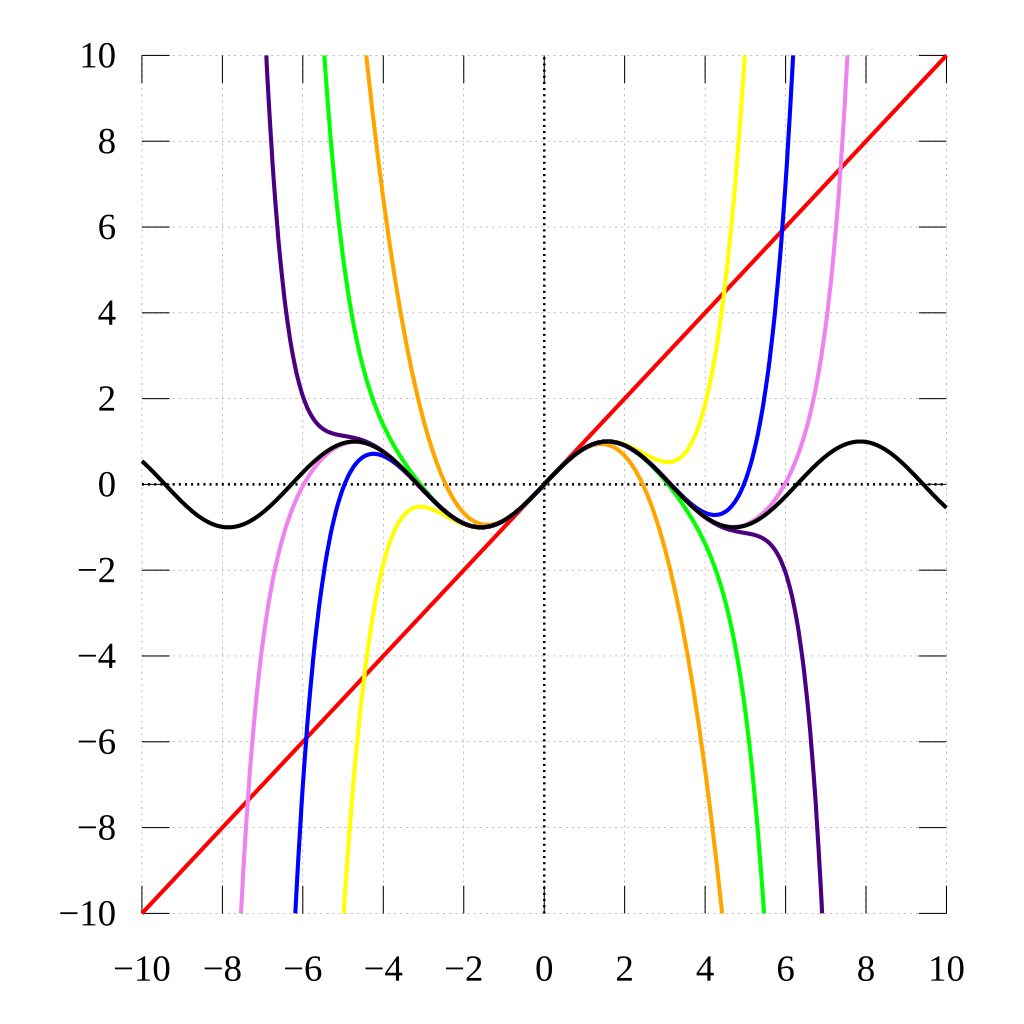
\includegraphics[width=0.5\linewidth]{figures/2background/taylor_exp.png}
    \caption{Given $f(x) = \sin(x)$, as the degree of the Taylor expansion increases, it better approximates the function around our chosen point $x=0$. Shown here is the Taylor expansion of $f$ where $p \in [1,3,5,7,9,11,13]$ at $x=0$.}
    \label{fig:taylor_expansion}
\end{figure}

Second-order methods, as said in their name, use a second-order Taylor expansion (i.e., $p = 2$). In deep learning, we want to minimise the loss function $L$ given our current parameters $\theta$. This means we want to find a step $\Delta \theta$ such that $L(\theta + \Delta \theta) < L(\theta)$. We do this by taking a second-order Taylor expansion of $L$ at $\theta$ to approximate $L(\theta + \Delta \theta)$ as follows.
\begin{align}
    L(\theta + \Delta \theta) &\approx L(\theta) + \nabla L(\theta)^T (\theta + \Delta \theta - \theta) + \frac{1}{2} (\theta + \Delta \theta - \theta)^T \nabla^2 L(\theta) (\theta + \Delta \theta - \theta) \\
    &= L(\theta) + \nabla L(\theta)^T \Delta \theta + \frac{1}{2} \Delta \theta^T \nabla^2 L(\theta) \Delta \theta \\
    &= L(\theta) + g^T \Delta \theta + \frac{1}{2} \Delta \theta^T H \Delta \theta.
    \label{equation:quadratic_model_w_loss}
\end{align}

This gives our quadratic model $m$ in terms of $\Delta \theta$. We refer to this as $m(\Delta \theta)$ in this case as $\Delta \theta$ is our step here that we want to find, though we note that this can be generalised to any step $p$. If $H$ is positive definite, we then have a strictly convex quadratic function that we easily find the minimum of and thus solve for $\Delta \theta$. We do this by taking the derivative of the quadratic model with respect to $\Delta \theta$ and setting it to zero \citep{NoceWrig06}.
\begin{align}
    0 &= \nabla_{\Delta \theta} \left( L(\theta) + g^T \Delta \theta + \frac{1}{2} \Delta \theta^T H \Delta \theta \right) \\
    &= g + H \Delta \theta.
\end{align}
Now, we solve for $\Delta \theta$, in which we get that:
\begin{align}
    \Delta \theta = - H^{-1} g.
\end{align} 
This is known as the \textit{Newton step} \citep{NoceWrig06, cvbook, mml_book}. In the context of an optimisation algorithm, we iteratively solve for $\Delta \theta_t$ by considering our model $m_t(\Delta \theta_t)$ at an iteration $t$ with our current parameters $\theta_t$. This gives us \textit{Newton's method} \citep{NoceWrig06,cvbook,mml_book}.
\begin{align}
    \text{Solve } m_t(\Delta \theta_t) \text{ for } \Delta \theta_t \\
    \Delta \theta_t = -H_t^{-1} g_t, \\
    \theta_{t+1} = \theta_t + \Delta \theta_t.
\end{align}
where $H_t$ is the Hessian evaluated at $\theta_t$ and $g_t$ is as defined in \cref{equation:first_order_update}.

% TODO: Scale invariance diagram here. [FIXED]
The quadratic model and Newton's method are central to second-order optimisation methods. In particular, they offer a few key advantages over first-order methods. 
\begin{itemize}
    \item \textit{Local Curvature}: The quadratic model incorporates a more sophisticated understanding of the local curvature of the optimisation landscape compared to the gradient used by first-order methods, allowing for more informed steps.
    \item \textit{Analytical Solution}: The quadratic model can be minimised analytically with respect to $\Delta \theta$. This gives a candidate for the optimal step. 
    \item \textit{Scale Invariance}: The Newton step is \textit{scale-invariant}. This means its performance is not adversely affected by linear rescaling of the parameters $\theta$ \citep{NoceWrig06}. This is because it rescales the problem space through the use of $H^{-1}$, which naturally adapts to the local curvature of the objective function. We show an example of this with the Rosenbrock function in \cref{fig:scale_invariance}.
    This property makes Newton's method very effective for ill-conditioned problems, as mentioned before in \cref{ssec:ill_conditioning_nonsmooth}. It can navigate elongated valleys or surfaces with disparate scaling across more effectively than first-order methods.
    \item \textit{Quadratic Convergence}: The Newton step exhibits \textit{quadratic convergence} \citep{NoceWrig06, cvbook}. Given that $H$ is positive definite, this means we can converge quadratically to a local minimum if we are sufficiently close to it. This is much faster than first-order methods which have linear or sub-linear convergence rates \citep{NoceWrig06, cvbook, mml_book}.
\end{itemize}

\begin{figure}[h]
    \begin{subfigure}[b]{0.48\linewidth}
        \centering
        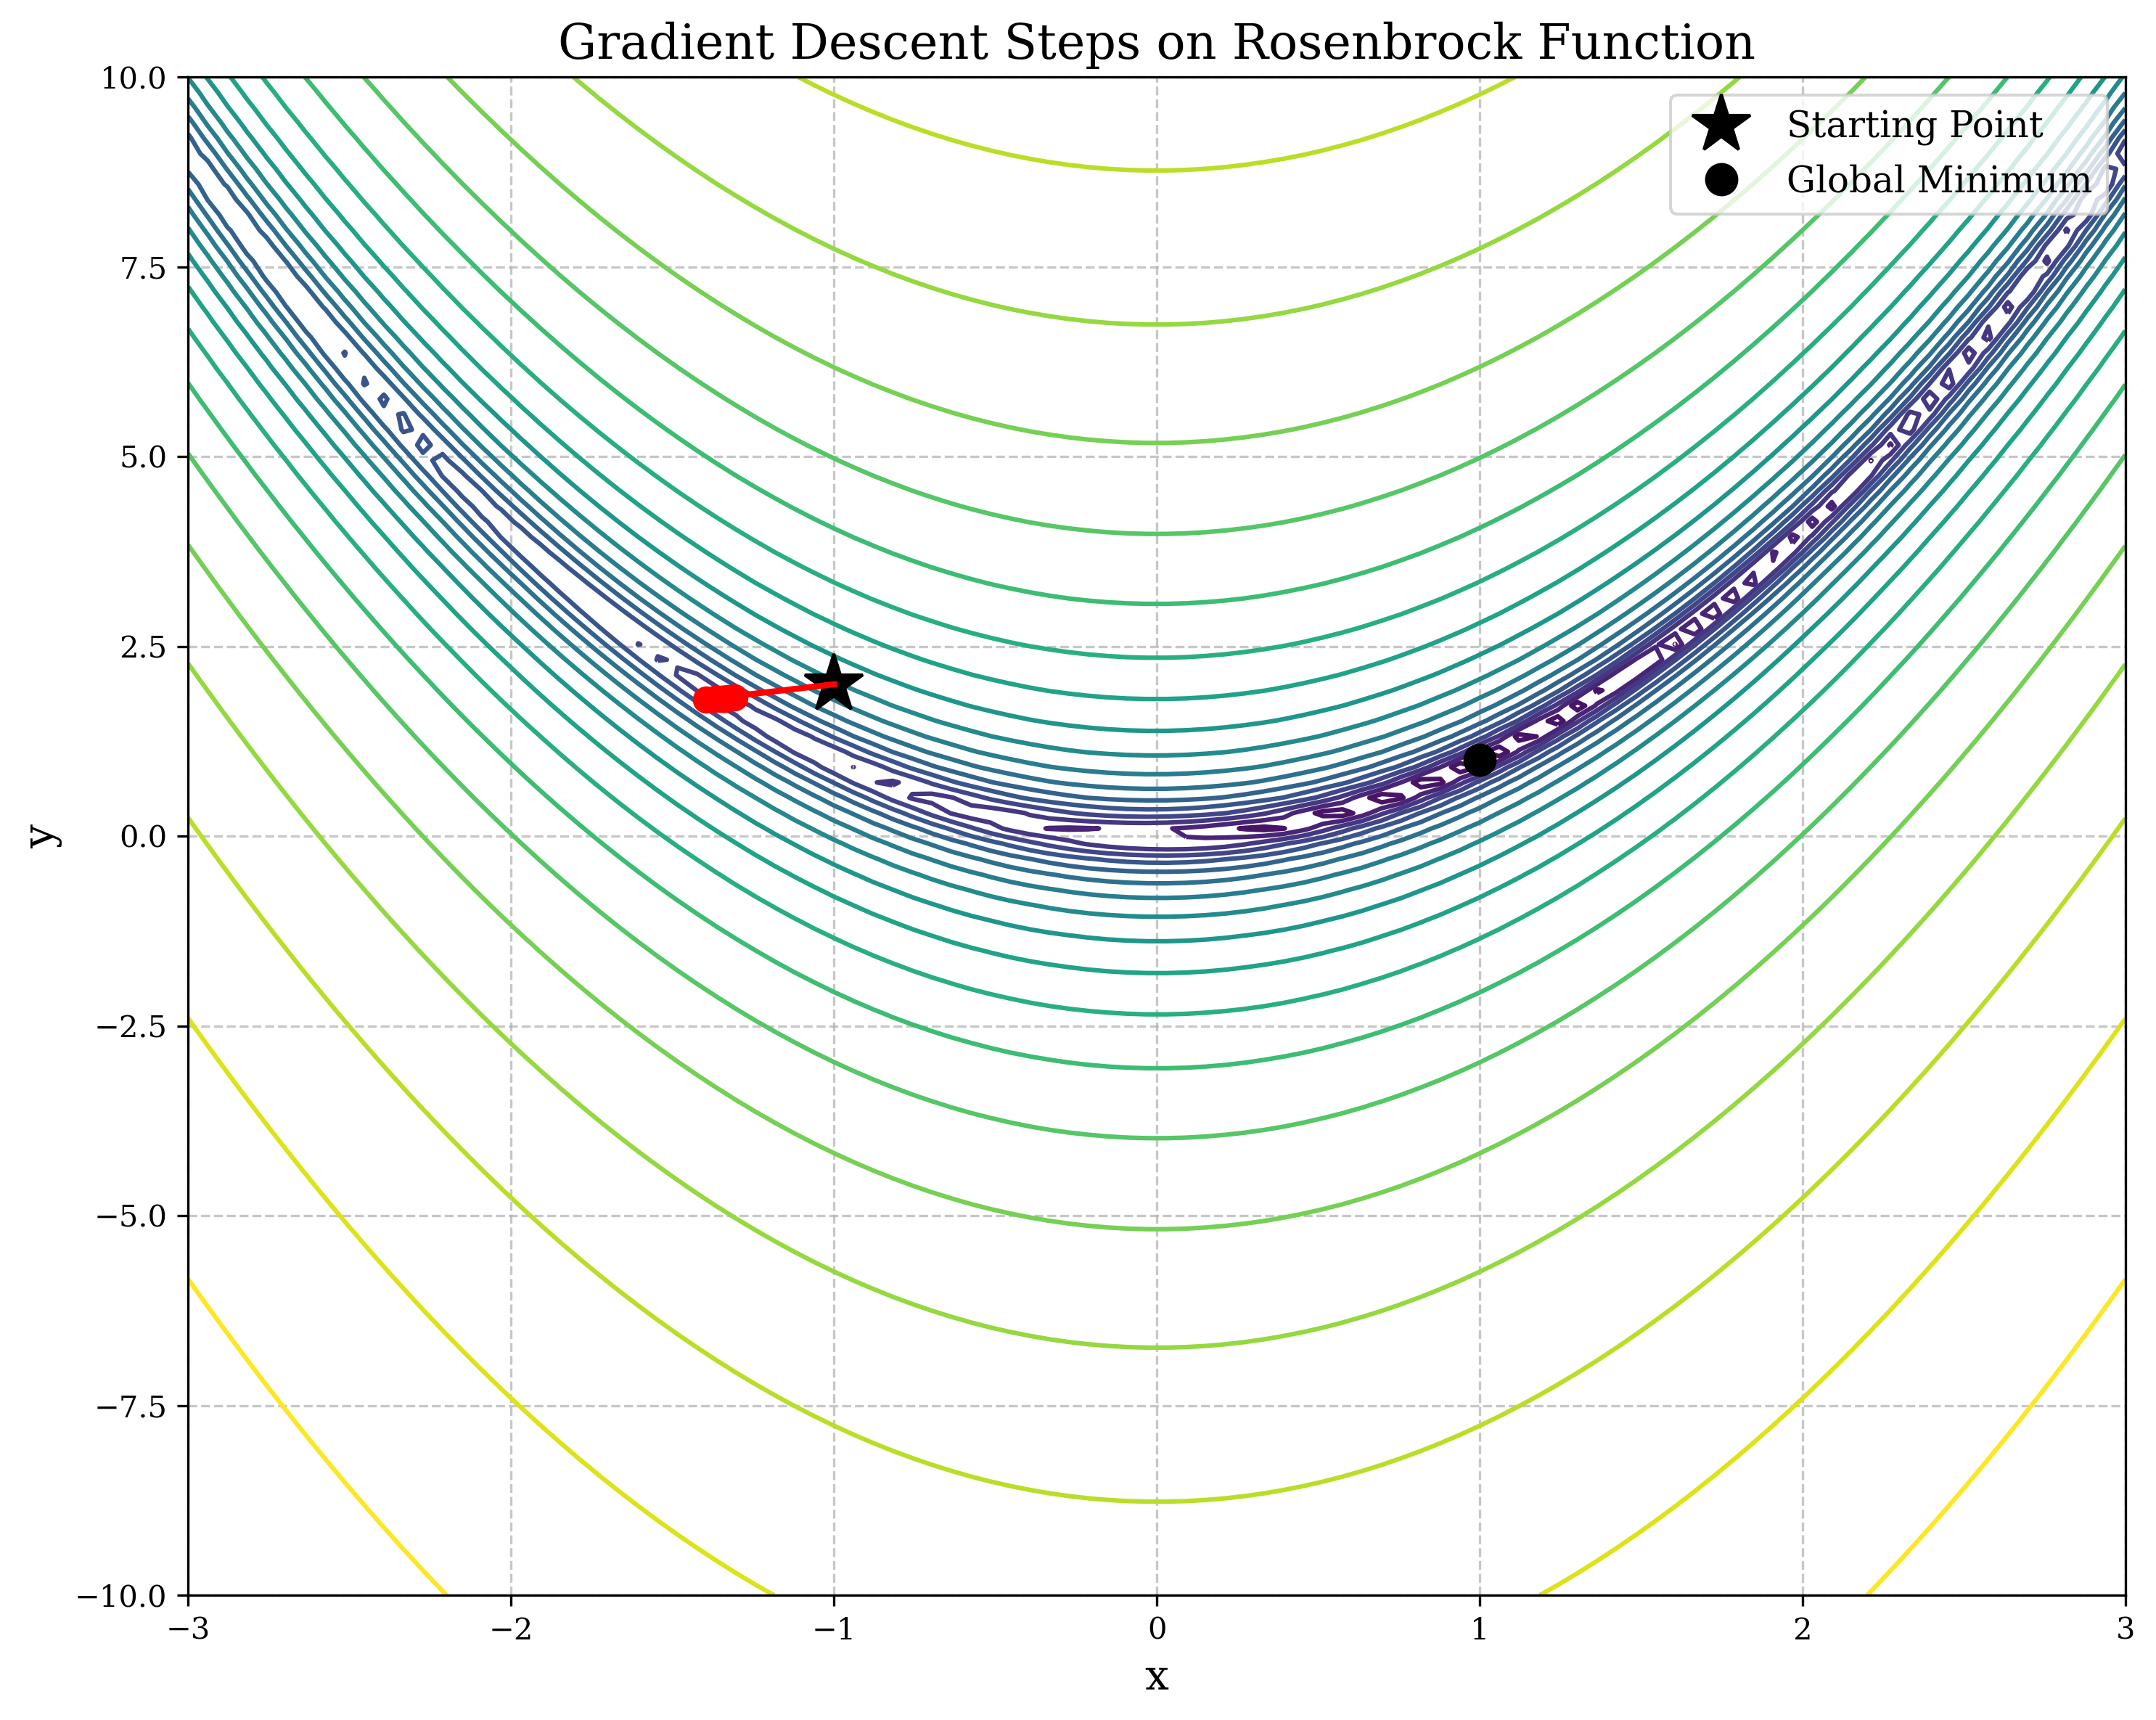
\includegraphics[width=\linewidth]{figures/2background/rosenbrock_gd.png}
        \caption{Trajectory of steepest descent on the Rosenbrock function with $\alpha = 0.01$.}
        \label{fig:rosenbrock_gd}
    \end{subfigure}
    \hfill
    \begin{subfigure}[b]{0.48\linewidth}
        \centering
        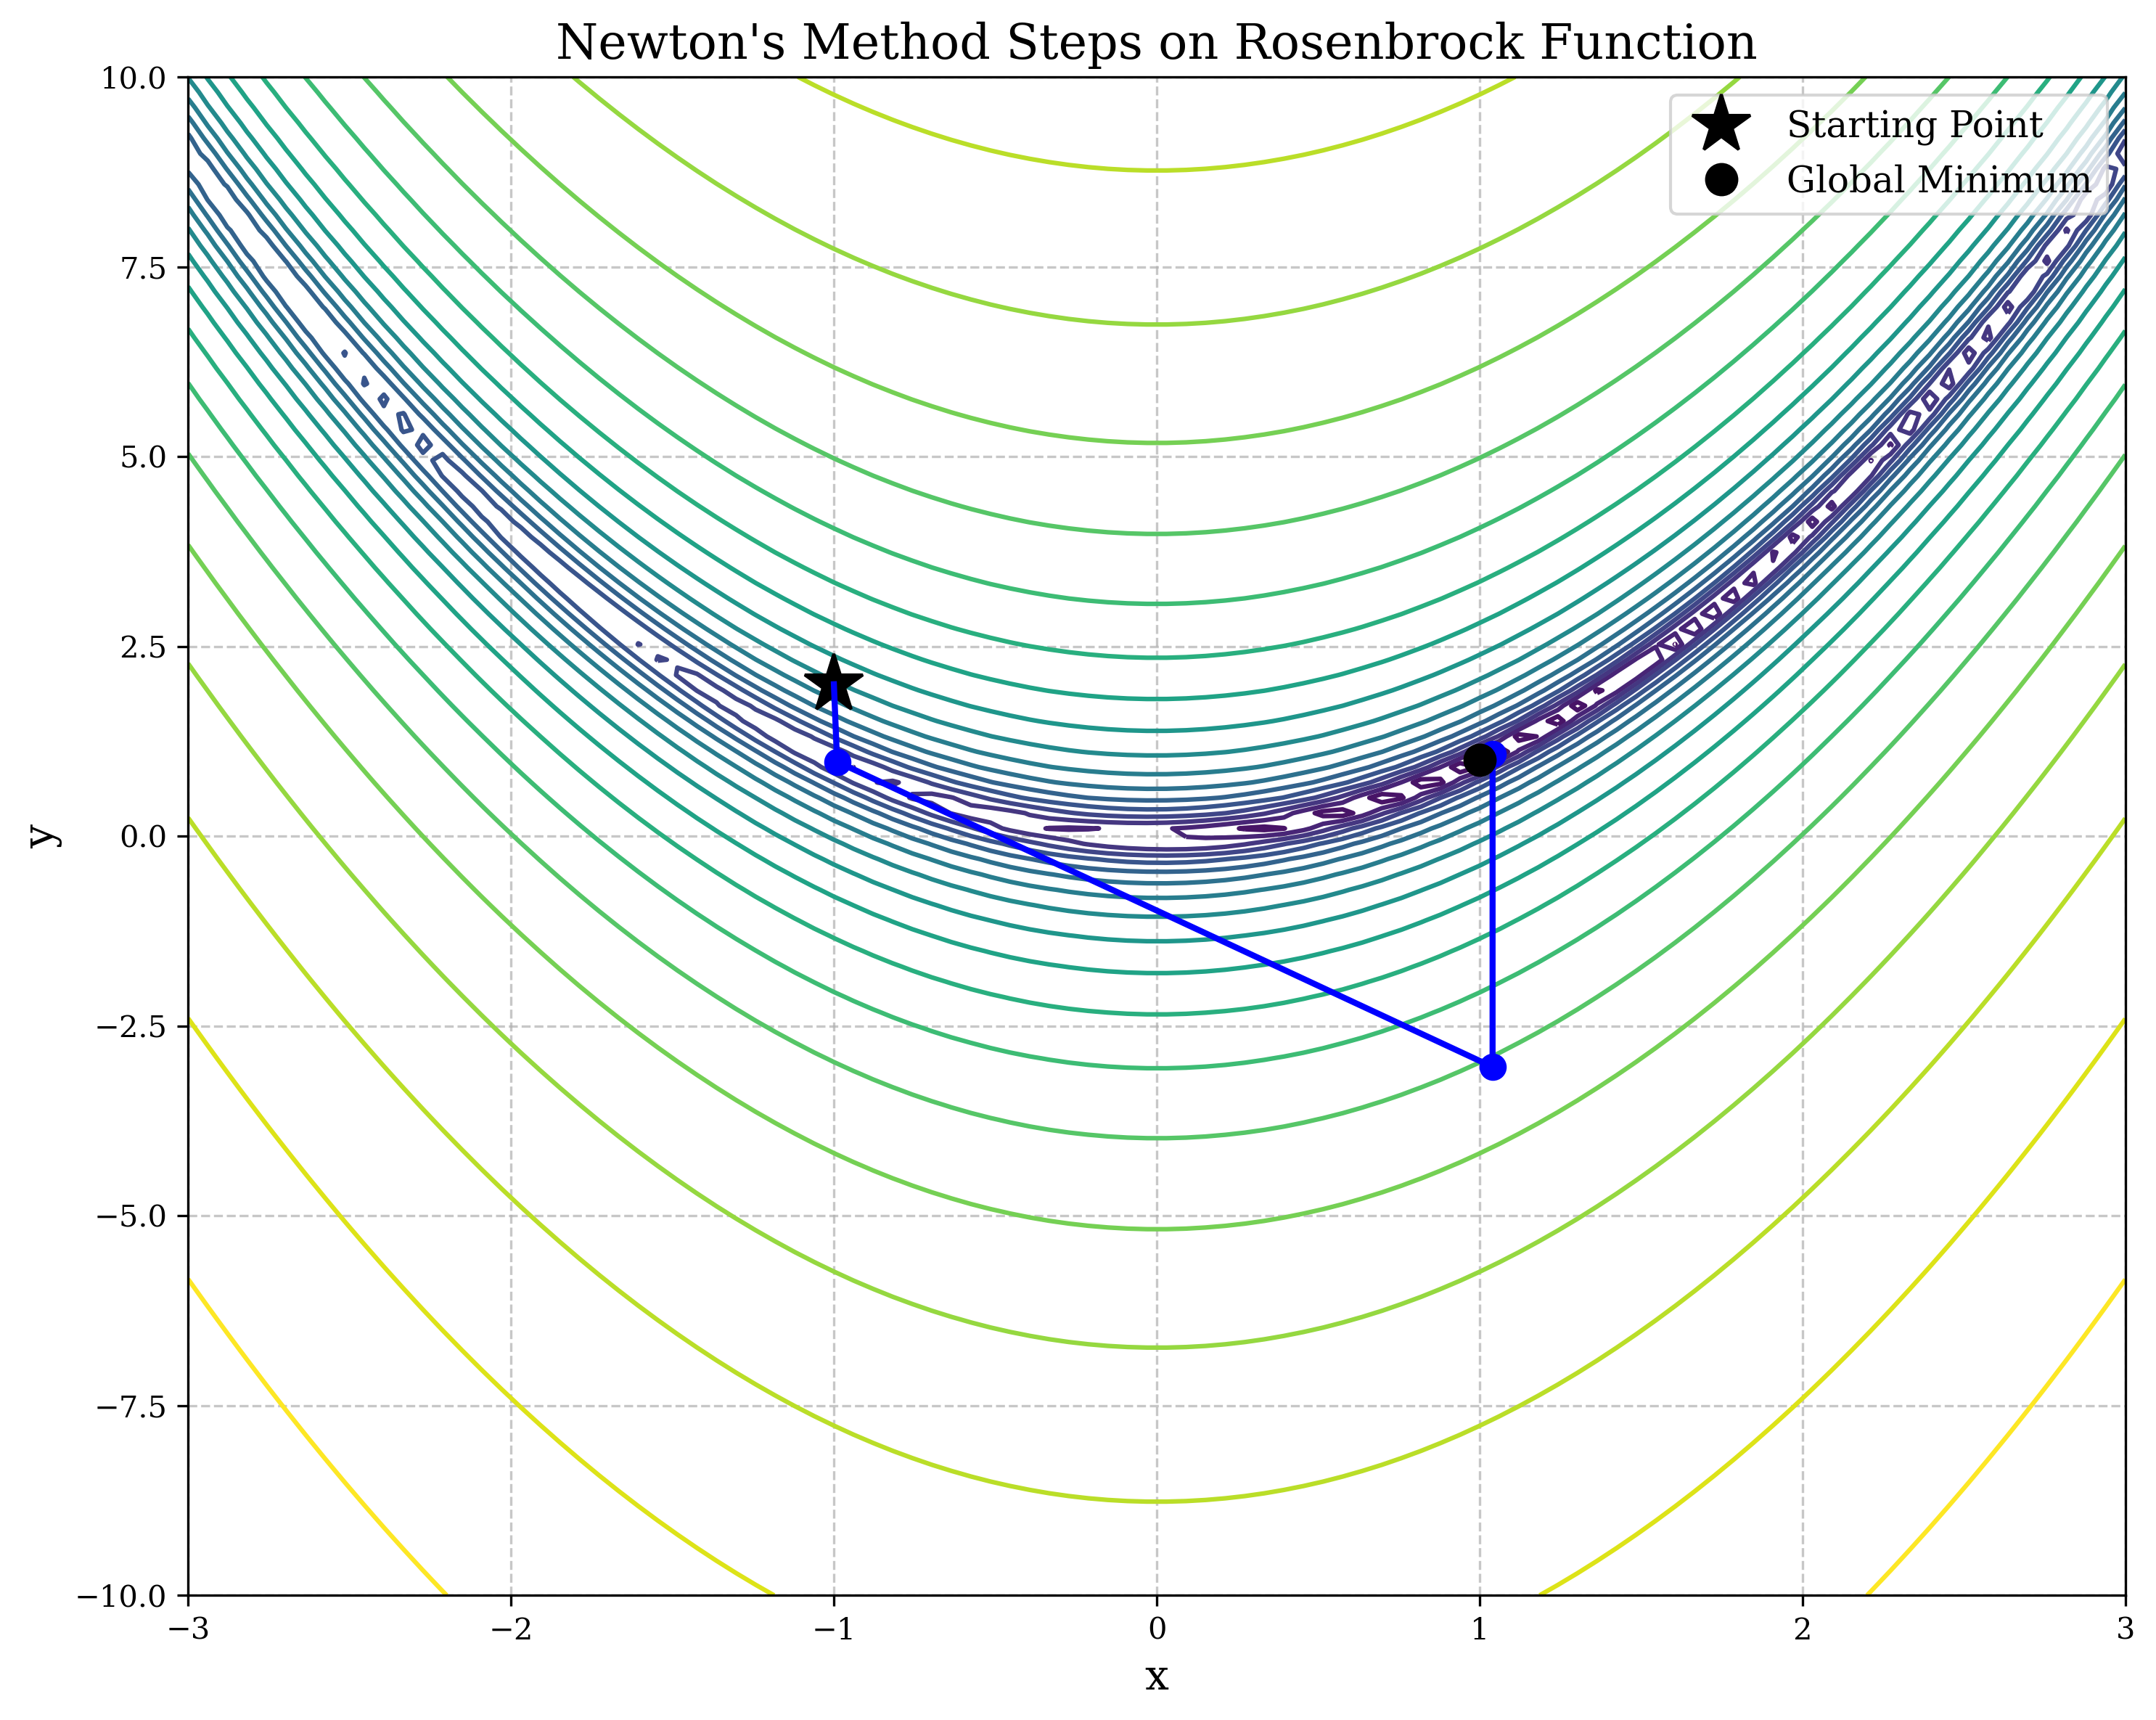
\includegraphics[width=\linewidth]{figures/2background/rosenbrock_newton.png}
        \caption{Trajectory of Newton's method on the Rosenbrock function.}
        \label{fig:rosenbrock_newton}
    \end{subfigure}
    \caption{Steepest descent and Newton's method on the Rosenbrock function for 10 steps. We see that the optimising using steepest descent direction makes slow progress, while Newton's method converges quickly in the first few steps.}
    \label{fig:scale_invariance}
\end{figure}

However, despite these advantages, second-order methods face challenges in deep learning. This is primarily due to their computation cost. The first challenge is the storing the Hessian matrix $H$. As $H$ is an $N \times N$ matrix, it requires $O(N^2)$ space to store \citep{deep_learning_book}. This is infeasible to compute with large-scale models, which are very common in deep learning. The second challenge is the computation of $H^{-1}$, required for methods such as Newton's method. This requires $O(N^3)$ computation time. Additionally matrix inversion is difficult to parallelise and thus is not as friendly on modern GPU hardware \citep{deep_learning_book}. This is significant since most of modern deep learning relies heavily on GPU parallelisation and distributed computing \citep{pytorch}. As such, the difficulty of pure Newton-style methods makes it impractical for large-scale deep learning. We note that this does not mean methods that rely on the quadratic approximation or inverse Hessian are useless, as there exist tractable methods that approximate them to capture local curvature. We discuss these in \Cref{sec:tractable_curvature_exploitation} and \Cref{chap:lit_review}.

Beyond computational demands and their constraints, there is one significant problem with the Newton method, which is that it is \textit{attracted} to saddle points \citep{dauphin2014sfn}. Consider the classic horse saddle $f(x, y) = x^2 - y^2$ as introduced in \cref{fig:horse_saddle}. To understand the behaviour of Newton's method, we can examine how it acts along each of the two principal directions. 
\begin{itemize}
    \item Along the $x$-axis, we have the component function $g(x) = x^2$. 
    \item Along the $y$-axis, we have the component function $h(y) = -y^2$.
\end{itemize}
Suppose we minimise $g(x)$ with Newton's method. We get that the gradient is $\nabla g(x) = 2x$ and the Hessian is $H_g = \nabla^2 g(x) = 2$ in the $x$-direction given we take the derivatives with respect to $x$. Then, the inverse Hessian is $\frac{1}{2}$. For a point $x_0$, we compute the Newton step to get the next iterate $x_1$ as follows:
\begin{align}
    x_1 = x_0 + \Delta x = x_0 - H_g^{-1} \nabla g(x_0) = x_0 - \frac{1}{2} \cdot 2 x_0 = 0.
\end{align}
This correctly moves us to the local minimum of $g(x)$ at $x = 0$, and we only take one step to do this which demonstrates the fast convergence of Newton's method, especially given that $g(x)$ is convex. 

Now, we consider the behaviour along the $y$-axis for $h(y)$. The gradient is $\nabla h(y) = -2y$ and the Hessian is $H_h = \nabla^2 h(y) = -2$ in the $y$-direction given we take the derivatives with respect to $y$. The inverse Hessian is now $-\frac{1}{2}$. For a point $y_0$, if we compute the Newton step to get $y_1$, we observe the following.
\begin{align}
    y_1 = y_0 + \Delta y = y_0 - H_h^{-1} \nabla h(y_0) = y_0 - \left(-\frac{1}{2} \cdot -2 y_0\right) = y_0 - y_0 = 0.
\end{align}
In this case, the Newton step has taken us towards the \textit{local maximum} of $h(y)$ at $y = 0$. We see that the Newton step actually goes in the wrong direction and does not minimise the function, which would involve taking the negative gradient direction as is done with gradient descent. As a result, our next set of iterates $(x_1, y_1)$ are $(0, 0)$, the exact point that is a saddle for our original function $f$. If we then try to take a step from here, we will still remain at $(0, 0)$ as our gradient will be $0$. Thus, we get stuck at the saddle point. We illustrate this in \cref{fig:newton_attract}.

\begin{figure}[h]
    \begin{subfigure}[b]{0.33\linewidth}
        \centering
        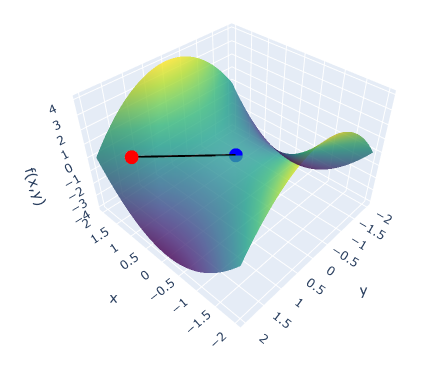
\includegraphics[width=\linewidth]{figures/2background/attract1.png}
        \caption{The Newton step on the 2D horse saddle function.}
        \label{fig:2d_attract}
    \end{subfigure}
    \hfill
    \begin{subfigure}[b]{0.32\linewidth}
        \centering
        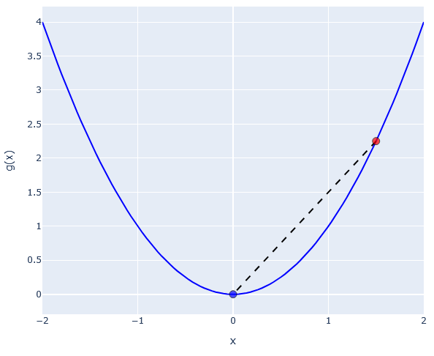
\includegraphics[width=\linewidth, height=100px]{figures/2background/attract2.png}
        \caption{The Newton step on the $x$-axis component.}
        \label{fig:x_attract}
    \end{subfigure}
    \hfill
    \begin{subfigure}[b]{0.33\linewidth}
        \centering
        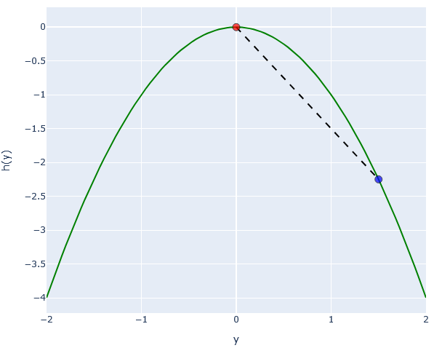
\includegraphics[width=\linewidth, height=100px]{figures/2background/attract3.png}
        \caption{The Newton step on the $y$-axis component.}
        \label{fig:y_attract}
    \end{subfigure}
    \caption{Newton's method on the classic 2D horse saddle function. Given a starting point $(1.5, 1.5)$ in red, the Newton step is attracted towards the saddle points at $(0, 0)$ in blue. We see that for the $x$-axis component, it correctly minimises the component function $g(x)$, but for the $y$-axis component, it moves away from the minima instead.}
    \label{fig:newton_attract}
\end{figure}

This is because Newton's method is attracted to saddle points when $H$ is indefinite \citep{dauphin2014sfn}. In this example, the eigenvalues of $H$ correspond to being $\lambda_1 = 2$ and $\lambda_2 = -2$. Intuitively, this means that along positive eigenvalue directions, the Newton step correctly moves towards minima, but along negative eigenvalue directions, it \textit{moves away from the minima}. When $H$ is instead negative definite, the Newton step will move towards the local maximum instead as our function is locally concave at the current point. This is a significant concern given the proliferation of saddle points we discussed in \cref{ssec:dl_challenges}. 

While it may seem like Newton's method and the quadratic model approximation are not a good fit for deep learning, multiple variants have extended these core ideas and have found success. These include \textit{damped Newton} methods, \textit{Quasi-Newton} methods, and \textit{diagonal Hessian} approximations \citep{NoceWrig06, liu2023sophia}. We discuss these further in the next section and provide a detailed review in \cref{chap:lit_review}.

\section{Methods for Tractable Curvature Exploitation}
\label{sec:tractable_curvature_exploitation}

In this section, we discuss strategies that can incorporate curvature information while being computationally tractable. We start by discussing \textit{Hessian-vector} products in \cref{ssec:hessian_vector_products}. This is followed by an introduction to Krylov subspaces in \cref{ssec:krylov_subspaces} and then trust-region methods in \cref{ssec:trust_region_methods}.

\subsection{Hessian-vector Products}
\label{ssec:hessian_vector_products}

We saw previously in \cref{ssec:second_order_methods} that storing the Hessian matrix $H$ or computing its inverse $H^{-1}$ is infeasible in deep learning due to computational constraints. However, many optimisation algorithms incorporate curvature information without explicitly forming the Hessian. One way to do this is through \textit{Hessian-vector} products \citep{pearlmutter1994fast,bloghvp}.

\begin{definition}[Hessian-vector Product]
    Given a loss function $L(\theta)$ with parameters $\theta \in \mathbb{R}^N$, the Hessian-vector product of $H = \nabla^2 L(\theta)$ with a vector $v \in \mathbb{R}^N$ is defined as:
    \begin{align}
        Hv = \nabla^2 L(\theta) \cdot v, 
    \end{align}
    where $Hv \in R^N$.
\end{definition}
We abbreviate Hessian-vector products as HVPs from here onwards. Intuitively, the HVP captures how $g$ changes when we move in a specific direction $v$. It captures the local curvature of the optimisation landscape in this direction. The key insight is that we can compute HVPs efficiently without explicitly forming $H$ by considering the directional derivative of $g$ with respect to $v$. Instead of requiring $O(N^2)$ time and space, HVPs can be computed with only two gradient evaluations \citep{pearlmutter1994fast, bloghvp, martens2010hessianfree}. This is known as Pearlmutter's trick.

\begin{definition}[Pearlmutter's Trick for Efficient HVPs] The HVP is the directional derivative of $g$ in the direction $v$,
\begin{align}
    Hv = \lim_{\epsilon \to 0} \frac{1}{\epsilon}[\nabla L(\theta + \epsilon v) - \nabla L(\theta)] = \nabla[\langle\nabla L(\cdot), v\rangle](\theta), 
\end{align} 
where $\langle \cdot, \cdot \rangle$ denotes the standard Euclidean inner product. See that this follows from the standard definition of the directional derivative for differentiable functions.
\end{definition}
Based on this identity, HVPs can be computed efficiently with automatic differentiation systems using only $O(N)$ computation and storage \citep{pytorch}. This makes them comparable to standard gradient calculations. HVPs are valuable for deep learning optimisation as they provide access to curvature information while remaining computationally tractable. Modern deep learning frameworks implement HVPs efficiently using automatic differentiation modes such as \textit{forward-mode} and \textit{reverse-mode} \citep{pytorch,henriques2019small}. This allows for easy integration with deep learning tasks.

HVPs form the foundation of many iterative algorithms. We discuss these more generally in \cref{chap:lit_review}, and in the next section introduce the notion of Krylov subspaces, which leverages matrix-vector products like HVPs to allow for efficient optimisation.

\subsection{Krylov Subspaces}
\label{ssec:krylov_subspaces}

In \cref{ssec:dl_challenges}, we discussed the challenges of the high-dimensional landscapes present in deep learning. In \cref{ssec:second_order_methods}, we followed this by discussing the problem of evaluating $H$ or $H^{-1}$. We now introduce \textit{Krylov subspaces}, which are a powerful iterative method that addresses these challenges \citep{NoceWrig06,krylov_book}.

Consider a general linear system $Ax = b$ where $A \in R^{N \times N}$, and $x, b \in R^{N}$. In a high-dimensional system where $N \gg 1$, solving this is difficult and often intractable. An example of this is the Newton step, $\Delta \theta = H^{-1} g$, where we outlined this as a core limitation in the previous section. However, one way to approximate them is to replace the $N$-dimensional space with a much lower dimensional space $M$ where $M \ll N$. This is the essence of Krylov subspaces.

\begin{definition}[Krylov Subspace]
    Given an $N \times N$ matrix $A$ and a vector $u \in R^N$ where $u \neq 0$, we define the $M$-th \textit{Krylov matrix} $K_M \in R^{N \times M}$ as
    \begin{align}
        K_M(A, u) = \begin{bmatrix} u & A u & A^2 u & \cdots & A^{M-1} u \end{bmatrix}.
        \label{eq:krylov_matrix}
    \end{align}
    Then, the subspace spanned by the columns of $K_M(A, u)$ is called the $M$-th \textit{Krylov subspace}, $\mathcal{K}_M(A, u)$:
    \begin{align}
        \mathcal{K}_M(A, u) = \text{span} \{u, A u, A^2 u, \ldots, A^{M-1} u \}.
    \end{align}
\end{definition}

Generally, $\mathcal{K}_M$, which is the \textit{rank} of $K_M$, equals $M$, though it may be smaller \citep{bloghvp}. Krylov matrices and their subspaces possess the following mathematical properties.
\begin{definition}[Properties of Krylov Matrices and Krylov Subspaces]
    Given the $M$-th Krylov matrix $K_M(A, u)$ and the $M$-th Krylov subspace $\mathcal{K}_M(A, u)$ generated by $A \in \mathbb{R}^{N \times N}$ and $u \in \mathbb{R}^N$, if we have an $x \in \mathcal{K}_M$, then following properties hold:
    \begin{itemize}
        \item $x = K_M z$ for some $z \in \mathbb{R}^M$.
        \item $x \in K_{M+1}$.
        \item $A x \in \mathcal{K}_{M+1}$.
        \item $\mathcal{K}_M \subseteq \mathcal{K}_{M+1}$, and so Krylov subspaces are nested.
    \end{itemize}
    \label{definition:krylov_properties}
\end{definition}

The appeal of generating $\mathcal{K}_M$ lies in its reliance on matrix-vector products $A v$, which can be computed efficiently. In general, the Krylov subspace can be stored with $O(M N)$ space for a Krylov dimension $M$ \citep{NoceWrig06, pytorch}. We can now solve our original problem $Ax = b$ by equivalently replacing $x$ with $K_M z$ as described above.
\begin{align}
    \min_{x \in \mathcal{K}_M} \| A x - b \| = \min_{z \in \mathbb{R}^M} \| A (K_M z) - b \| = \min_{z \in \mathbb{R}^M} \| (A K_M) z - b \|.
    \label{equation:krylov_subspace_problem}
\end{align}
This is a much lower dimensional problem which we can solve efficiently.
Note that the natural seed vector for this problem is $b$, and so we can equivalently solve this in the Krylov subspace $\mathcal{K}_M(A, b)$.

While the columns of $K_M$ in \cref{eq:krylov_matrix} form a basis for $\mathcal{K}_M$, the basis is often ill-conditioned. This is especially the case as $M$ increases. This is because repeated matrix-vector products with matrix-powers $A^k$ tend to concentrate in the direction of the \textit{dominant eigenvector} of $A$ \citep{krylov_book}.
\begin{definition}[Dominant Eigenvector of Matrix-Powers]
    Given a matrix $A \in \mathbb{R}^{N \times N}$, suppose we have eigenvalues $\lambda_1, \lambda_2, \lambda_3, \ldots, \lambda_N$ such that 
    \begin{align}
        |\lambda_1| \geq |\lambda_2| \geq |\lambda_3| \geq \cdots \geq |\lambda_N|.
    \end{align}
    Then, for any vector $u \in \mathbb{R}^N$, $A^k u$ is eventually a scalar multiple of the \textit{dominant eigenvector} of $A$ as $k \to \infty$. The dominant eigenvector is the vector associated with the largest magnitude eigenvalue, $\lambda_1$.
\end{definition}

As such, when $M$ is large, each basis vector $A^k u$ in our Krylov subspace $\mathcal{K}_M$ is increasingly parallel to the dominant eigenvector of $A$. The basis vectors are thus increasingly linearly dependent and the condition number of $K_M$ deteriorates. To overcome this, we instead construct the opposite of an ill-conditioned basis, an orthonormal basis for $\mathcal{K}_M$. 

Consider \textit{QR factorisation}, which factorises a matrix $A$ into an orthogonal matrix $Q$ and an upper triangular matrix $R$ \citep{NoceWrig06}. We can then write $K_M$ as:
\begin{align}
K_M = \text{QR}(K_M) = Q_M R_M = [q_1, q_2, \ldots, q_M] 
\begin{bmatrix} 
R_{11} & R_{12} & \cdots & R_{1M} \\ 
0 & R_{22} & \cdots & R_{2M} \\ 
\vdots & \vdots & \ddots & \vdots \\ 
0 & 0 & \cdots & R_{MM}.
\end{bmatrix}
\end{align}

The vectors $q_1, q_2, \ldots, q_M$ are the orthonormal basis for $\mathcal{K}_M$. By \cref{definition:krylov_properties}, we know that $A q_M \in \mathcal{K}_{M+1}$, and therefore,
\begin{align}
A q_M = h_{1M} q_1 + h_{2M} q_2 + \cdots + h_{M+1,M} q_{M+1}
\label{equation:arnoldi_recurrence}
\end{align}
for some choice of the $h_{iM}$ coefficients. Using orthonormality, we have:
\begin{align}
q_i^T(A q_M) = h_{iM}, \quad i = 1,\ldots,M.
\label{equation:cij_projection}
\end{align}

We can then solve for $h_{M+1,M}$ and $q_{M+1}$ as these are the only unknowns in \cref{equation:arnoldi_recurrence}, since we started by assuming that we know $q_1, \ldots, q_M$. Given they appear as a product, and we know that $q_{M+1}$ is a unit vector due to orthonormality, they must be uniquely defined by the other terms in the equation. This results in the \textit{Arnoldi iteration} algorithm, which computes $Q_M$ \citep{krylov_book}. We outline this below in \cref{alg:arnoldi_iteration}.

\begin{algorithm}[H]
    \DontPrintSemicolon
    \KwIn{Matrix $\mathbf{A}$, vector $\mathbf{u}$, Krylov dimension $M$}
    \KwOut{Orthonormal basis $Q_M$ for $\mathcal{K}_M(A, u)$}
    $\mathbf{q}_1 \leftarrow \mathbf{u} / \|\mathbf{u}\|$\; 
    \For{$m=1, 2, \ldots, M$}{ 
        {Find $h_{im}$ for $i = 1,\ldots,m$ using \cref{equation:cij_projection}} \label{line:arnoldi_h_find} \\
        {Compute $\mathbf{v} = (A\mathbf{q}_m) - h_{1m} \mathbf{q}_1 - h_{2m} \mathbf{q}_2 - \cdots - h_{mm} \mathbf{q}_m$} via \cref{equation:arnoldi_recurrence} \label{line:arnoldi_v_def} \\
        $h_{m+1,m} \leftarrow \|\mathbf{v}\|$\;
        $\mathbf{q}_{m+1} \leftarrow \mathbf{v} / h_{m+1,m}$\;
    } 
    \caption{The Arnoldi Iteration}
    \label{alg:arnoldi_iteration}
\end{algorithm}

The Arnoldi iteration iteratively constructs nested orthonormal bases for nested Krylov subspaces. Although we have focused on finding $Q_M$, the $h_{ij}$, the coefficient values $h_{ij}$ are key. For $j = 1,2,\ldots,M$ in \cref{equation:arnoldi_recurrence} we get that

\begin{align}
AQ_M &= [Aq_1 \ldots Aq_M] \nonumber \\
&= [q_1 \ldots q_{M+1}]
\begin{bmatrix} 
h_{11} & h_{12} & \cdots & h_{1M} \\ 
h_{21} & h_{22} & \cdots & h_{2M} \\ 
       & h_{32} & \ddots & \vdots \\ 
       &        & \ddots & h_{M,M} \\
       &        &        & h_{M+1,M}
\end{bmatrix} \nonumber \\
&= Q_{M+1} H_M.
\label{equation:arnoldi_identity}
\end{align}

We call this the \textit{fundamental identity of Krylov subspaces} \citep{krylov_book}. The matrix $H_M$ is of size $M+1 \times M$ and has a special structure where $h_{ij} = 0$ whenever $i > j + 1$\footnote{This is usually the definition of an upper Hessenberg matrix. However $H_M$ is not square in our case since it has an extra row. If we remove the last row, then it becomes an upper Hessenberg matrix.}. Note that generally speaking, although we have used the similar notation, $H_M$ is not related to the Hessian $H$.

When we project $Q_M$ onto the original matrix $A$, we obtain a reduced system $Q_M^T A Q_M = H_M$ of size $M \times M$ \citep{krylov_book}. This is crucial as this acts as an approximation to the original matrix $A$, and thus the eigenvalues of $H_M$ are approximations to the eigenvalues of $A$. If we consider the case when $A$ is the Hessian $H$, then we can use this to approximate the Hessian eigenvalue spectrum and obtain local curvature information. As the Krylov dimension $M$ becomes closer to $N$, $H_M$ becomes a better approximation of $A$ \citep{krylov_book}. This property makes Krylov subspaces very powerful for optimisation, as we can work in this reduced subspace while still obtaining a good solution to our problem.

Krylov subspaces have been key in developing many successful numerical solvers and deep learning optimisers. For example, the \textit{Krylov Subspace Descent} algorithm can construct sound approximations and incorporate local curvature to perform well in deep learning tasks \citep{vinyals2012krylov}. We discuss these further in \cref{chap:lit_review}.

\subsection{Trust-Region Methods}
\label{ssec:trust_region_methods}

We finish this chapter by introducing \textit{trust-region methods}, another class of second-order optimisation algorithms that can utilise curvature information. Trust-region methods use the quadratic model as we discussed in \cref{ssec:second_order_methods} to define a \textit{region} around the current iterate that they \textit{trust} to be a good approximation of the objective function, hence the name \textit{trust-region} \citep{NoceWrig06}. 

We discussed the quadratic model in \cref{ssec:second_order_methods} in the specific case of deep learning. We defined it with respect to a loss function $L(\theta)$ and the model parameters $\theta$ using the explicit Hessian $H$. We now define the quadratic model in the general case to use for trust-region methods.

\begin{definition}[General Quadratic Model]
    Given an objective function $f: \mathbb{R}^N \to \mathbb{R}$, the quadratic model is the second-order Taylor expansion of $f$ around a point $x \in \mathbb{R}^N$,
    \begin{align}
    m(p) = f(x) + g^T p + \frac{1}{2} p^T B p,
    \label{eq:tr_quadratic_model}
    \end{align}
    where $g = \nabla f(x)$ is the gradient, and $B$ is a symmetric matrix that usually approximates the Hessian $\nabla^2 f(x)$.
\end{definition}
If we consider $f$ as the loss function $L(\theta)$ and $p$ as $\Delta \theta$, then this is the same as \cref{equation:quadratic_model_w_loss} when $B = H$. Trust-region methods employ this quadratic model to iteratively solve a \textit{constrained optimisation problem} that is the \textit{trust-region subproblem} \citep{NoceWrig06}. A constrained optimisation problem is one where we must adhere to constraints on our parameters \citep{cvbook}. Here, we optimise $f$ subject to the constraint that our step size $||p||$ is less then a given \textit{trust-region radius} $\Delta$.

\begin{definition}[The Trust-Region Subproblem]
    Given a function $f: \mathbb{R}^N \to \mathbb{R}$ and a trust-region radius $\Delta > 0$, the trust-region subproblem is to find a step $p$ that solves
    \begin{align}
        \min_{p \in \mathbb{R}^N} m(p) \quad \text{subject to} \quad \|p\| \leq \Delta,
        \label{eq:tr_subproblem}
    \end{align}
    where $\| \cdot \|$ is usually the Euclidean norm.
\end{definition}

The trust-region radius $\Delta$ controls the maximum size of our step $p$. It represents the region in which we trust our quadratic model to be a good approximation of the objective function. If $\Delta$ is too small, then we make little progress. If $\Delta$ is too large, our quadratic model we may overshoot and take a poor step. When we take a step $p$, we consider the ratio between the actual and prediction reduction in the objective function \citep{NoceWrig06}. We denote this ratio as $\rho$.
\begin{align}
    \rho = \frac{f(x) - f(x + p)}{m(0) - m(p)} = \frac{\text{actual reduction}}{\text{predicted reduction}},
    \label{eq:reduction_ratio}
\end{align}
For our step $p$, we want $\rho$ to be always non-negative, as this guarantees that $p$ is a descent direction \citep{NoceWrig06}. We can characterise the behaviour of the trust-region based on the value of $\rho$ as follows:
\begin{itemize}
    \item \textit{Rejection}: If $\rho$ is negative, then $f(x + p) > f(x)$ and so our step does not minimise the objective function. In this case, we \textit{reject} the step \citep{NoceWrig06}.
    \item \textit{Acceptance and Expansion}: If $\rho$ is close to 1, then our model $m$ is a good approximation of $f$ and we can accept $p$. If we also have that $\|p\| = \Delta$, then we \textit{expand} our trust-region radius $\Delta$ as this indicates that the step has reached the boundary of our trust-region \citep{NoceWrig06}.
    \item \textit{Acceptance and Shrinkage}: If $\rho$ is close to 0, then our model is a poor approximation of $f$ and we should \textit{shrink} our trust-region radius $\Delta$ \citep{NoceWrig06}.
\end{itemize}

To turn this into an optimisation algorithm, we iteratively solve the trust-region subproblem at the current iterate $x_t$ and update our trust-region radius $\Delta_t$. We illustrate the algorithm in \cref{alg:trust_region_algorithm}.

\begin{algorithm}[h]
    \DontPrintSemicolon
    \KwIn{Initial point $x_0$, initial trust-region radius $\Delta_0 > 0$, maximum radius $\hat{\Delta} > 0$, thresholds $0 < c_1 < c_2 < 1$, reduction factor $\gamma_1 \in (0,1)$, expansion factor $\gamma_2 > 1$, maximum iterations $T$}
    \KwOut{Approximate local minimiser $x_T$}
    $x \leftarrow x_0$\;
    $\Delta \leftarrow \Delta_0$\;
    \For{$t = 0, 1, 2, \ldots, T$}{
        Construct the quadratic model $m_t(p)$ in \cref{eq:tr_quadratic_model}\;
        Obtain $p_t$ by solving the trust-region subproblem in \cref{eq:tr_subproblem}\;
        Compute the ratio $\rho_t$ in \cref{eq:reduction_ratio}\;
        \uIf{$\rho_t < 0$}{ 
            $p_t \leftarrow 0$\; 
            $\Delta \leftarrow \gamma_1 \Delta$\; 
        }
        \uElseIf{$\rho_t < c_1$}{ 
            $\Delta \leftarrow \gamma_1 \Delta$\;
        }
        \uElseIf{$\rho_t > c_2$ \textbf{and} $\|p_t\| = \Delta$}{ 
            $\Delta \leftarrow \min(\gamma_2 \Delta, \hat{\Delta})$\;
        }
        $x_{t+1} \leftarrow x_t + p_t$\;
    }
    \Return{$x_{T}$}
    \caption{Trust-Region Method}
    \label{alg:trust_region_algorithm}
\end{algorithm}

The core of this algorithm is the trust-region subproblem. We discussed the solution to this in the deep learning case in \cref{ssec:second_order_methods} when $B = H$ to compute the Newton step. We also made an important note that the Newton step as a result of the quadratic model is not always a descent direction when $H$ is not positive semidefinite. We now adapt this for the general case, in which we want to solve
\begin{align}
    (B + \lambda I) p^* = -g,
    \label{eq:tr_subproblem_general}
\end{align}
where $\lambda \geq 0$ and $p^*$ is the solution. As a result the following conditions must be met if $p^*$ is the solution.

\begin{definition}[Trust-Region Subproblem Conditions]
    If $p^*$ is the solution to \cref{eq:tr_subproblem_general}, then the following\footnote{These are essentially the \textit{Karush-Kuhn-Tucker} (KKT) conditions for the trust-region subproblem.} must be satisfied:
    \begin{itemize}
        \item $\|p^*\| \leq \Delta$.
        \item $B + \lambda I$ is positive semidefinite.
        \item $\lambda (\Delta - \|p^*\|) = 0$.
    \end{itemize}
    \label{definition:tr_subproblem_conditions}
\end{definition}

These conditions characterise the exact solution, but solving this exactly is computationally expensive as discussed in \cref{ssec:second_order_methods}. In practice, we use approximation methods. A popular approach for approximately solving the trust-region subproblem is \textit{two-dimensional subspace optimisation}, where we restrict ourselves to a low dimensional subspace \citep{NoceWrig06}. We now have that 
\begin{align}
    \min_{p \in \mathcal{S}} m(p) \quad \text{subject to} \quad \|p\| \leq \Delta,
    \label{eq:subspace_tr_subproblem}
\end{align}
where $\mathcal{S} = \text{span}\{-g, B^{-1}g\}$ is the two-dimensional subspace \citep{NoceWrig06}. The first direction, $-g$, is the steepest descent direction which guarantees reduction. The second direction $B^{-1}g$ is also a solution when $B$ is positive definite. In the case it is not, we can then change the subspace to be $\text{span}\{-g, (B + \alpha I)^{-1}g\}$ where $\alpha \geq \lambda_{min}(B)$. Intuitively, this searches for a solution that is a linear combination of the descent direction \textit{and} the approximate Newton direction. Since we operate in subspace of size $2$, this becomes extremely inexpensive to solve. Subspace optimisation often is close to the exact solution of \cref{eq:tr_subproblem_general}. We can also extend two-dimensional subspace optimisation to higher dimensions. For example, it may be beneficial to find a solution within the subspace $\text{span}\{-g, B^{-1}g, z\}$ where $z$ is an average of past gradients (known as the momentum). 

With appropriate choices of $B$, trust-region methods poses strong convergence guarantees. These include:
\begin{itemize}
    \item \textit{Global Convergence}: Trust-region methods converge globally to stationary points regardless of the starting point, given $B$ is uniformly bounded and $g$ is Lipschitz continuous \citep{NoceWrig06} \footnote{A function is Lipschitz continuous if there exists a constant $L$ such that the slope between any two points is bounded by $L$, meaning the function cannot change too rapidly anywhere in its domain}.
    \item \textit{Protection against negative curvature}: Given we have a model approximation that we trust around a radius, we are protected against directions of negative curvature that might cause to diverge. This is since we will always stop at the boundary of the trust region.
    \item \textit{Second-order necessary conditions}: When $B = H$, trust-region methods guarantee convergence to points satisfying the second-order necessary conditions as seen in \cref{definition:second_order_necessary} \citep{NoceWrig06}.
    \item \textit{Superlinear or quadratic convergence}: Trust-region methods achieve superlinear or quadratic convergence rates near solutions satisfying second-order sufficient conditions as seen in \cref{definition:second_order_sufficient}, when using accurate Hessian approximations.
\end{itemize}

These properties make trust-region methods particularly useful in deep learning, as they offer a good balance between rapid progress, stability, and computational efficiency. 

% To summarise, we illustrate a trust-region method in action in \cref{fig:tr_example}.

% \begin{figure}[h]
%     \begin{subfigure}[b]{0.32\linewidth}
%         \centering
%         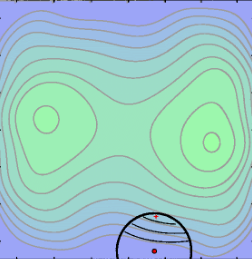
\includegraphics[width=\linewidth]{figures/2background/tr1.png}
%         \caption{We initialise a trust region. The model approximation is good, so we accept and expand.}
%         \label{fig:tr_example_1}
%     \end{subfigure}
%     \hfill
%     \begin{subfigure}[b]{0.32\linewidth}
%         \centering
%         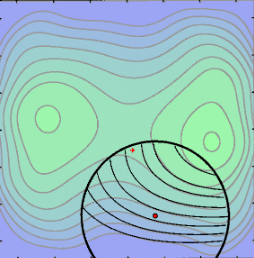
\includegraphics[width=\linewidth]{figures/2background/tr2.png}
%         \caption{At our new point, the model approximation is still good, so we accept and expand once more.}
%         \label{fig:tr_example_2}
%     \end{subfigure}
%     \hfill
%     \begin{subfigure}[b]{0.32\linewidth}
%         \centering
%         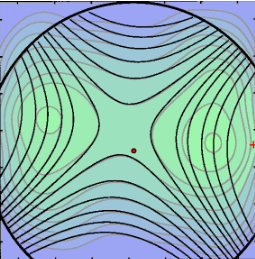
\includegraphics[width=\linewidth]{figures/2background/tr3.png}
%         \caption{The computed step does not reduce the objective function as the radius is too large, so we reject and shrink.}
%         \label{fig:tr_example_3}
%     \end{subfigure}
    
%     \vspace{1em}
    
%     \begin{subfigure}[b]{0.33\linewidth}
%         \centering
%         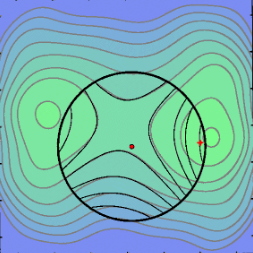
\includegraphics[width=\linewidth]{figures/2background/tr4.png}
%         \caption{Now, the model approximation is reasonable, so we accept and keep the radius.}
%         \label{fig:tr_example_4}
%     \end{subfigure}
%     \begin{subfigure}[b]{0.33\linewidth}
%         \centering
%         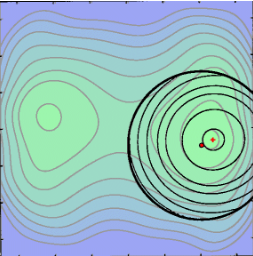
\includegraphics[width=\linewidth]{figures/2background/tr5.png}
%         \caption{We have now reached near a local minima. We can converge to it as the final step.}
%         \label{fig:tr_example_5}
%     \end{subfigure}
%     \caption{An example scenario of a trust-region method. We start at the red point and initialise a trust region, and adaptively expand and shrink the radius as we move along the contours of the objective function, evaluating our model approximation at each step until we reach a local minima.}
%     \label{fig:tr_example}
% \end{figure}

In this chapter, we have covered a complete overview on the fundamentals of optimisation, optimisation in deep learning, and how to efficiently incorporate curvature information for optimisation algorithms. We now discuss these algorithms and perform a comprehensive literature review of the state-of-the-art and foundational methods.